\documentclass{beamer}

\usepackage{framed}
\usepackage{graphicx}

\usepackage{amsmath}

\begin{document}
%======================================= %

\begin{frame}
	\Large
	\noindent\textbf{About ggplot}
	\bigskip
	
	\textbf{ggplot} is a graphics package for Python that aims to approximate \texttt{R}'s ggplot2 package in both usage and aesthetics.\\
	\bigskip
	\textbf{Authors:} Greg Lamp and Austin Ogilvie
\end{frame}
%======================================= %


\begin{frame}
	\begin{figure}
		\centering
		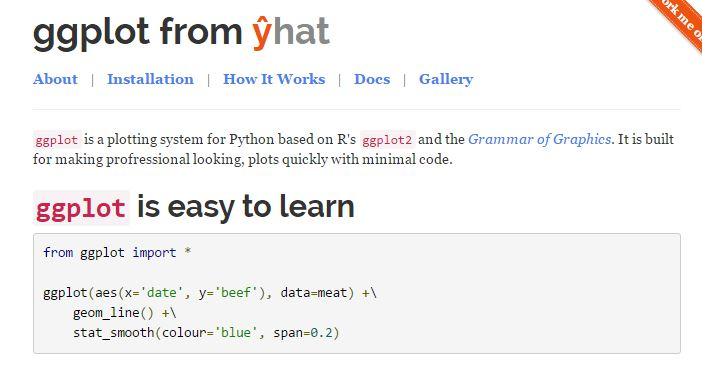
\includegraphics[width=1.1\linewidth]{ggplot-yhat}
	\end{figure}
	\Large
	\noindent \textbf{Important :} \\ For Python, the name is simply ``\textbf{ggplot}".
\end{frame}
%========================================== %
\begin{frame}
	\Large
	\noindent\textbf{What are Yhat saying?}
	
	\begin{enumerate}
		\item ggplot is easy to learn [\textit{1}]
		\item ggplot is fun
		\item ggplot is powerful [\textit{2}]
	\end{enumerate}
	
	\begin{framed}
		\textit{[1] Lots of learning resources, mainly intended for the R environment, that can applied to Python also.}\\
		\bigskip
		\textit{[2] Less code required to compute high-level publication quality plot}
	\end{framed}
\end{frame}	
%======================================== %	
\begin{frame}
	\begin{figure}
\centering
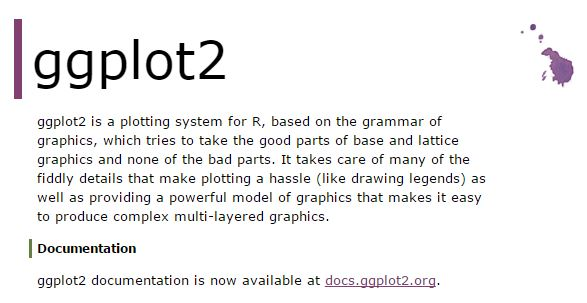
\includegraphics[width=1.1\linewidth]{ggplot2-website}
\end{figure}
website: www.had.co.nz

\end{frame}
%======================================== %
\begin{frame}
	\begin{figure}
\centering
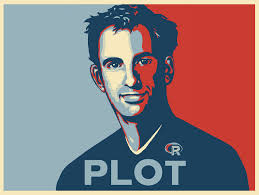
\includegraphics[width=0.95\linewidth]{HW}

\end{figure}
Hadley Wickham (Chief Data Scientist, RStudio)
\end{frame}
%============================================= %

\begin{frame}
\begin{figure}
\centering
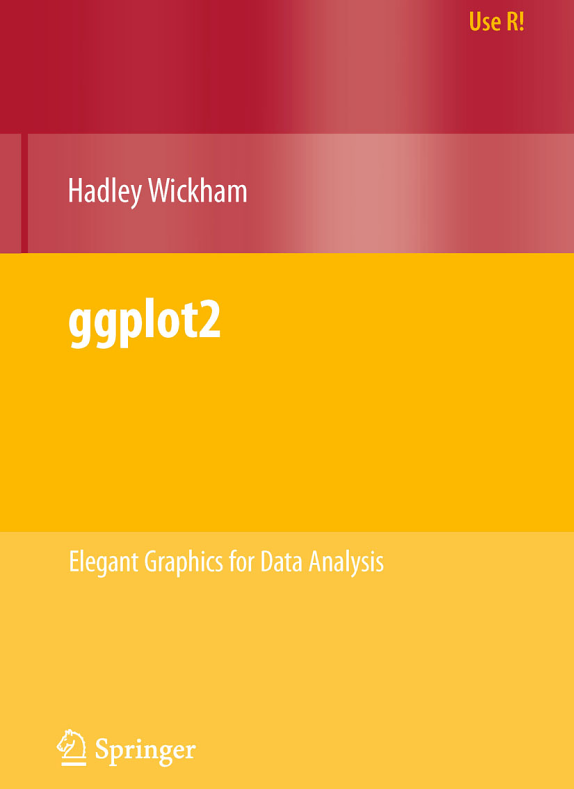
\includegraphics[width=0.55\linewidth]{ggplot2-bookcover}
\end{figure}
ggplot2: Elegant Graphics for Data Analysis
\end{frame}

%============================================= %

\begin{frame}
	
\begin{figure}
\centering

\includegraphics[width=0.8\linewidth]{yhat}
\end{figure}
\Large
\textbf{Yhat} (\textit{pronounced y-hat}) is a data science technology company that provides tools and systems that allow enterprises to turn data insights into data-driven products.\\ \bigskip


\end{frame}

%===================================== %
\begin{frame}[fragile]
\textbf{1. Installing ggplot}
\begin{framed}
\begin{verbatim}
pip install ggplot
\end{verbatim}
\end{framed}
N.B. Not loaded automatically with Anaconda, unlike pandas and numpy\\
\bigskip
\textbf{2. Getting Set Up on Jupyter Notebook}
\begin{figure}
\centering
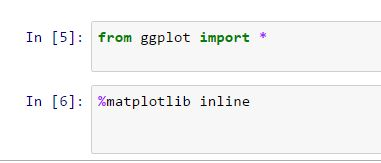
\includegraphics[width=0.7\linewidth]{jupyter1}
\end{figure}

\end{frame}
%===================================== %
\begin{frame}
	\Large
	\begin{figure}
\centering
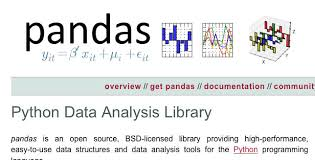
\includegraphics[width=0.7\linewidth]{pandas}
\end{figure}

	\textbf{Important:} ggplot accepts data in the form of a \texttt{pandas Dataframe}, so you need to configure all data accordingly first.
\end{frame}
%================================================================================== %
\begin{frame}[fragile]
	\frametitle{Data}
	\Large
	\begin{itemize}
		\item ggplot has a symbiotic relationship with pandas. 
		\item If you're planning on using ggplot, it's best to keep your data in DataFrames. 
		\item Think of a DataFrame as a tabular data object. 
%		\item For example, let's look at the diamonds dataset which ships with ggplot.
	\end{itemize}
\end{frame}
%================================================================================== %

\begin{frame}
	\frametitle{ggplot - Inbuilt Data Sets}
	\Large
	The ggplot package contains these inbuilt  pandas \texttt{DataFrame}.
	\begin{itemize}
		\item diamonds
		\item meat  (also: derived data set called meat2)
		\item movies
		\item mtcars
		\item pageviews
	\end{itemize}
	\bigskip
	\noindent \textbf{Remark:}
	ggplot code will work on any pandas \texttt{DataFrame}. 
\end{frame}
%===================================== %
\begin{frame}[fragile]
	\Large
	\begin{framed}
		\begin{verbatim}
		import pandas as pd
		
		meat2 = pd.melt(meat, id_vars=['date'])
		\end{verbatim}
	\end{framed}
\end{frame}


%================================================================================== %
\begin{frame}[fragile]
	\begin{framed}
		\begin{verbatim}
		from ggplot import *
		diamonds.head()
		\end{verbatim}
	\end{framed}
	\begin{figure}
		\centering
		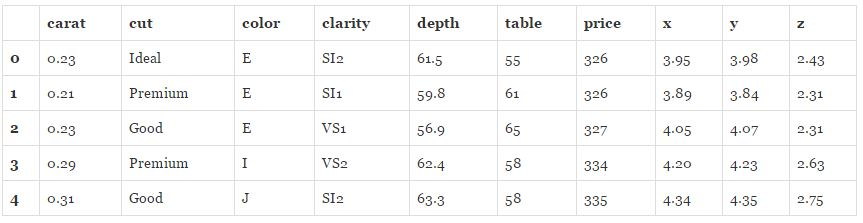
\includegraphics[width=1.1\linewidth]{diamondsdata}
		
	\end{figure}
	
\end{frame}	
%===================================== %
\begin{frame}[fragile]
	\Large

	\begin{figure}
\centering
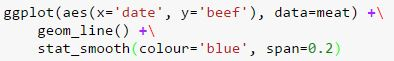
\includegraphics[width=1.05\linewidth]{plusoperator}
\end{figure}
\end{frame}
%===================================== %
\begin{frame}[fragile]
\Large
\noindent \textbf{For \texttt{R}  Users}
\begin{itemize}
	\item  In Python, dataframe columns (i.e. variables) are specified with quotation marks
\item Watch out for this operator
\begin{framed}
	\begin{verbatim}
	.... +\ .....
	\end{verbatim}
\end{framed}
\end{itemize}
\end{frame}
%===================================== %
\begin{frame}[fragile]
\Large
\begin{itemize}
\item The main command is \texttt{ggplot()}.
\item The name comes from "\textbf{grammar of graphics}", a book by Leland Wilkinson
\item A very ``high-level" approach to data visualization.
\end{itemize}
\begin{framed}
\begin{quote}
	A grammar of graphics is a tool that enables us to concisely describe the components
	of a graphic. Such a grammar allows us to move beyond named graphics (e.g., the “scatterplot”)
	and gain insight into the deep structure that underlies statistical graphics.
\end{quote}
\end{framed}
\end{frame}

\begin{frame}

\begin{figure}
\centering
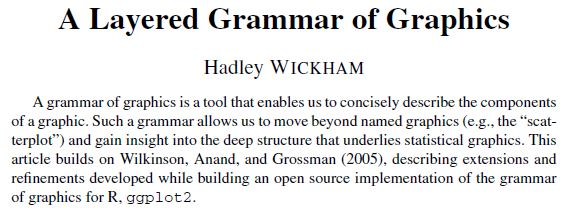
\includegraphics[width=1.1\linewidth]{HWpaper}
\end{figure}
\begin{framed}
Hadley Wickham.\\
\textbf{A layered grammar of graphics.}\\
\textit{Journal of Computational and Graphical Statistics, \\ vol. 19, no. 1, pp. 3–28, 2010.}
\end{framed}

\end{frame}

\section{How it works}
\begin{frame}[fragile]
	\Large
	\frametitle{Basic Premise}

	\begin{itemize}
		\item Making plots is a very repetive: draw this line, add these colored points, then add these, etc. 
		\item Instead of re-using the same code over and over, \texttt{ggplot} implements them using a high-level but very expressive API.
		\item The result is less time spent creating your charts, and more time interpreting what they mean.
	\end{itemize}
\textit{(From ggplot documentation)}	
\end{frame}

%================================================================================== %
\begin{frame}[fragile]
	\Large
\frametitle{Basic Premise}
	\begin{itemize}
		\item \texttt{ggplot} is not a good fit for people trying to make highly customized data visualizations. 
		\item \textit{(Compare this to high level ``Bokeh" plots)}
		\item While you can make some very intricate, great looking plots, \texttt{ggplot} sacrifices highly customization in favour of general doing "what you'd expect".
	\end{itemize}
\textit{(From ggplot documentation)}	
\end{frame}

%===================================== %
\begin{frame}[fragile]
	\begin{figure}
		\centering
		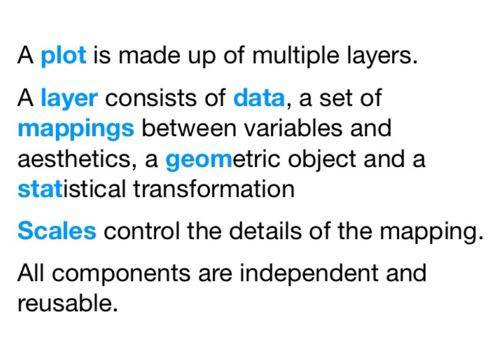
\includegraphics[width=1.1\linewidth]{ggplot2-info}
	\end{figure}
	(Source: Hadley Wickham)
\end{frame}
%================================================================================== %

\section{Layers}
\begin{frame}[fragile]
	\frametitle{Layers}
	\Large
	\noindent \textbf{Layers}
	\begin{itemize}
		\item \textbf{ggplot} lets you combine or add different types of visualization components (or layers) together. 
		%\item I think this is easiest to understand with an example.
		\item The command \texttt{ggplot} does not actually create any plot, rather it prepares a ``blank canvas" for further plotting 
		\item We will introduce \textit{geoms} shortly
	\end{itemize}
	
\end{frame}
%================================================================================== %
\begin{frame}[fragile]
\textbf{	Start with a blank canvas.}
	\begin{framed}
		\begin{verbatim}
		p = ggplot(aes(x="date", y="beef"), data=meat)
		p
		\end{verbatim}
	\end{framed}
	\begin{figure}
		\centering
		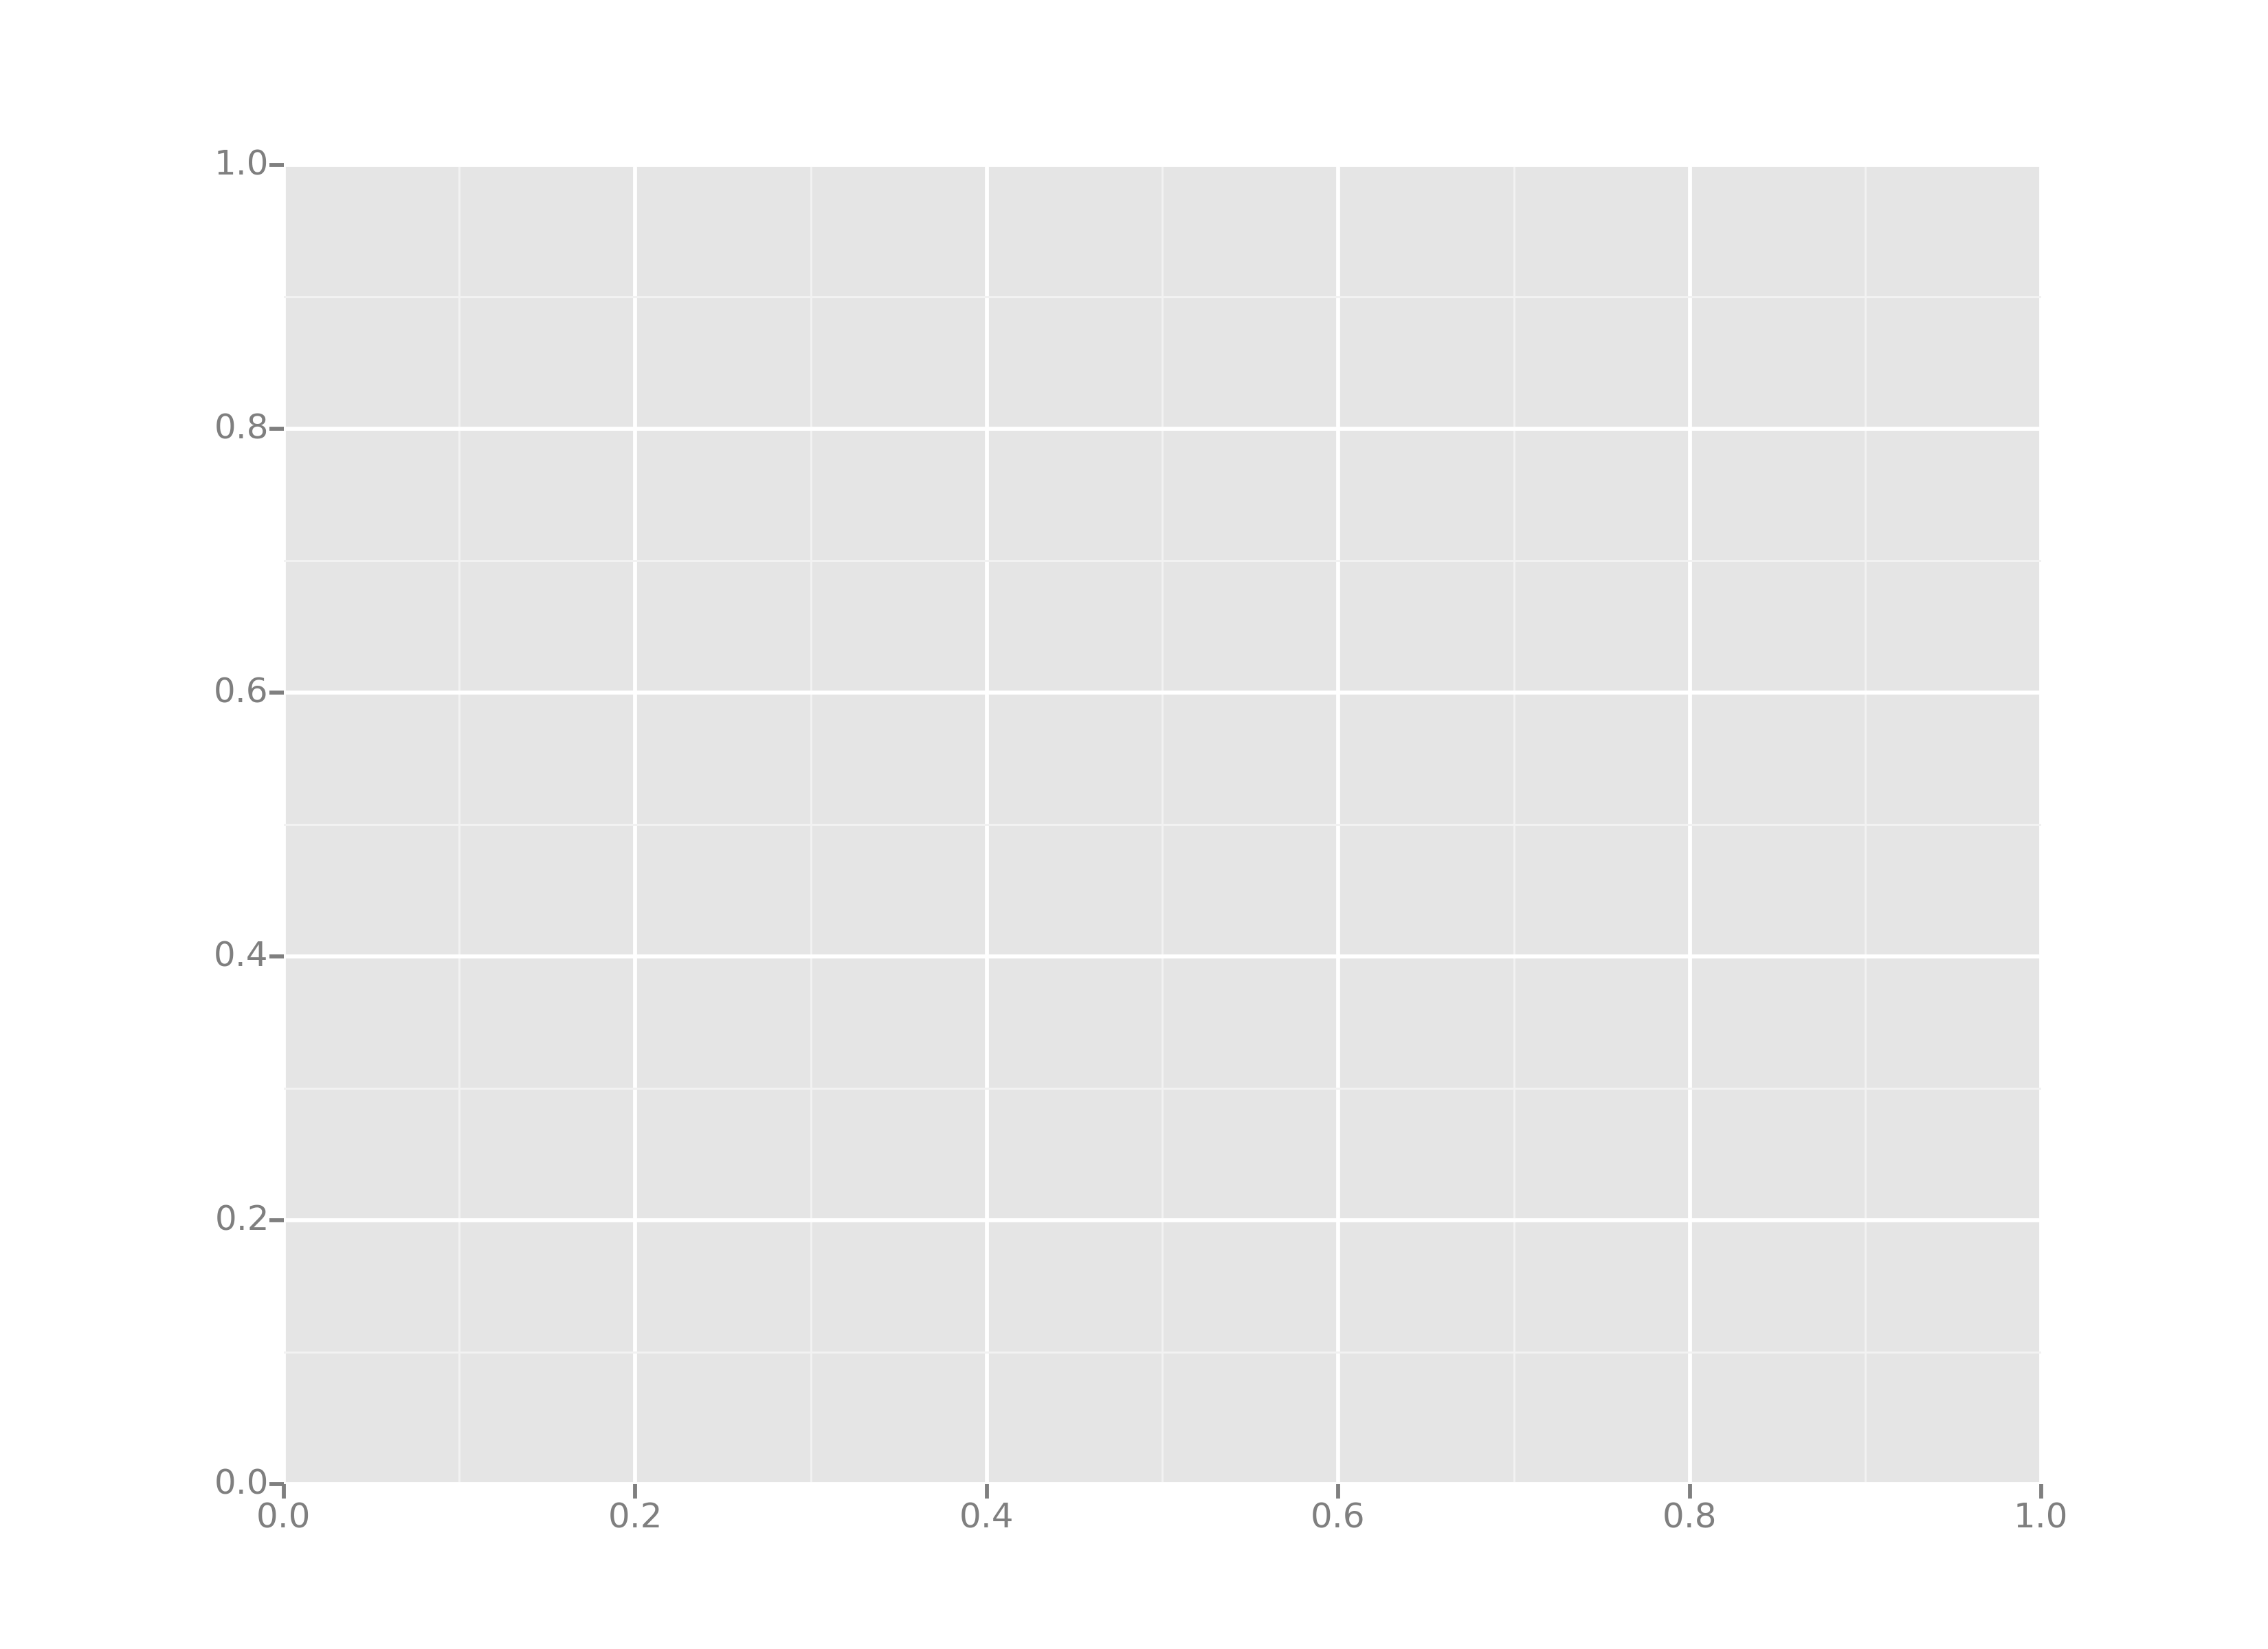
\includegraphics[width=0.7\linewidth]{Layers1}
	\end{figure}
	
\end{frame}
%================================================================================== %
\begin{frame}[fragile]
\textbf{	Add some points.}
	\begin{framed}
		\begin{verbatim}
		p + geom_point()
		\end{verbatim}
	\end{framed}
	\begin{figure}
		\centering
		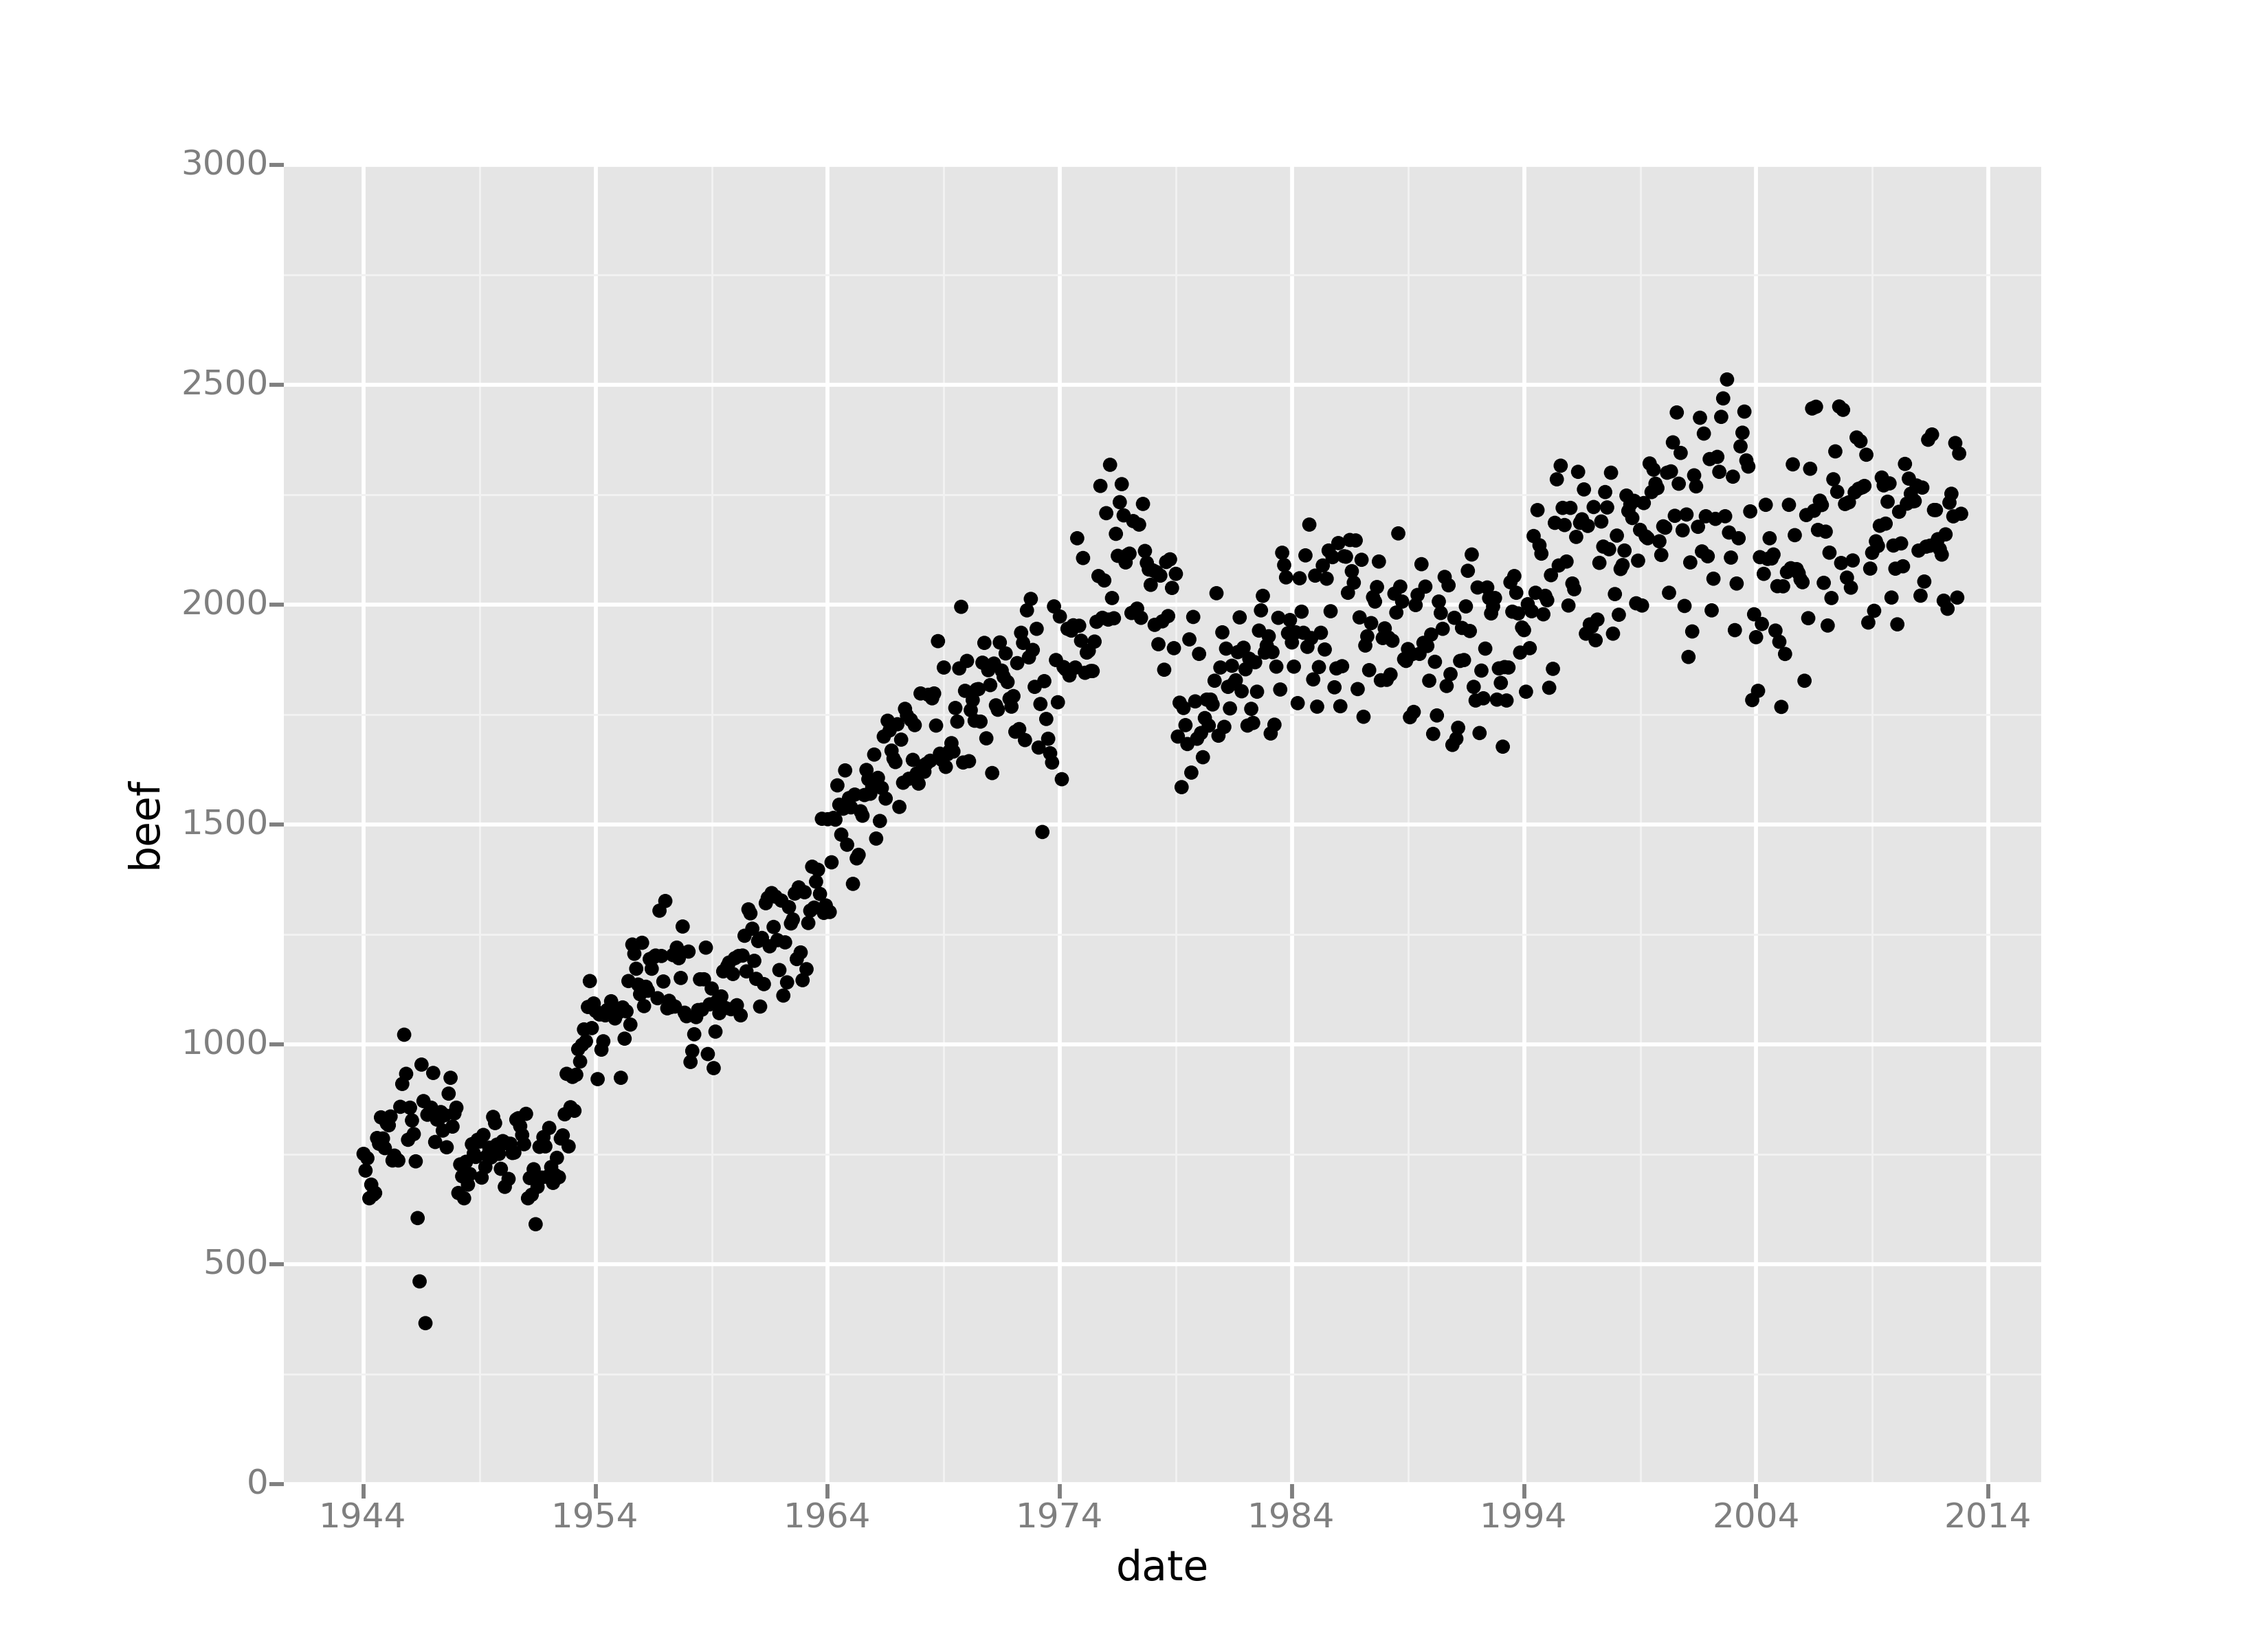
\includegraphics[width=0.7\linewidth]{Layers2}
	\end{figure}
	
	
\end{frame}
\begin{frame}[fragile]
%	\frametitle{ ggplot - Layers}
\textbf{	Add a line.}
	\begin{framed}
		\begin{verbatim}
		p + geom_point() + geom_line()
		\end{verbatim}
	\end{framed}
	\begin{figure}
		\centering
		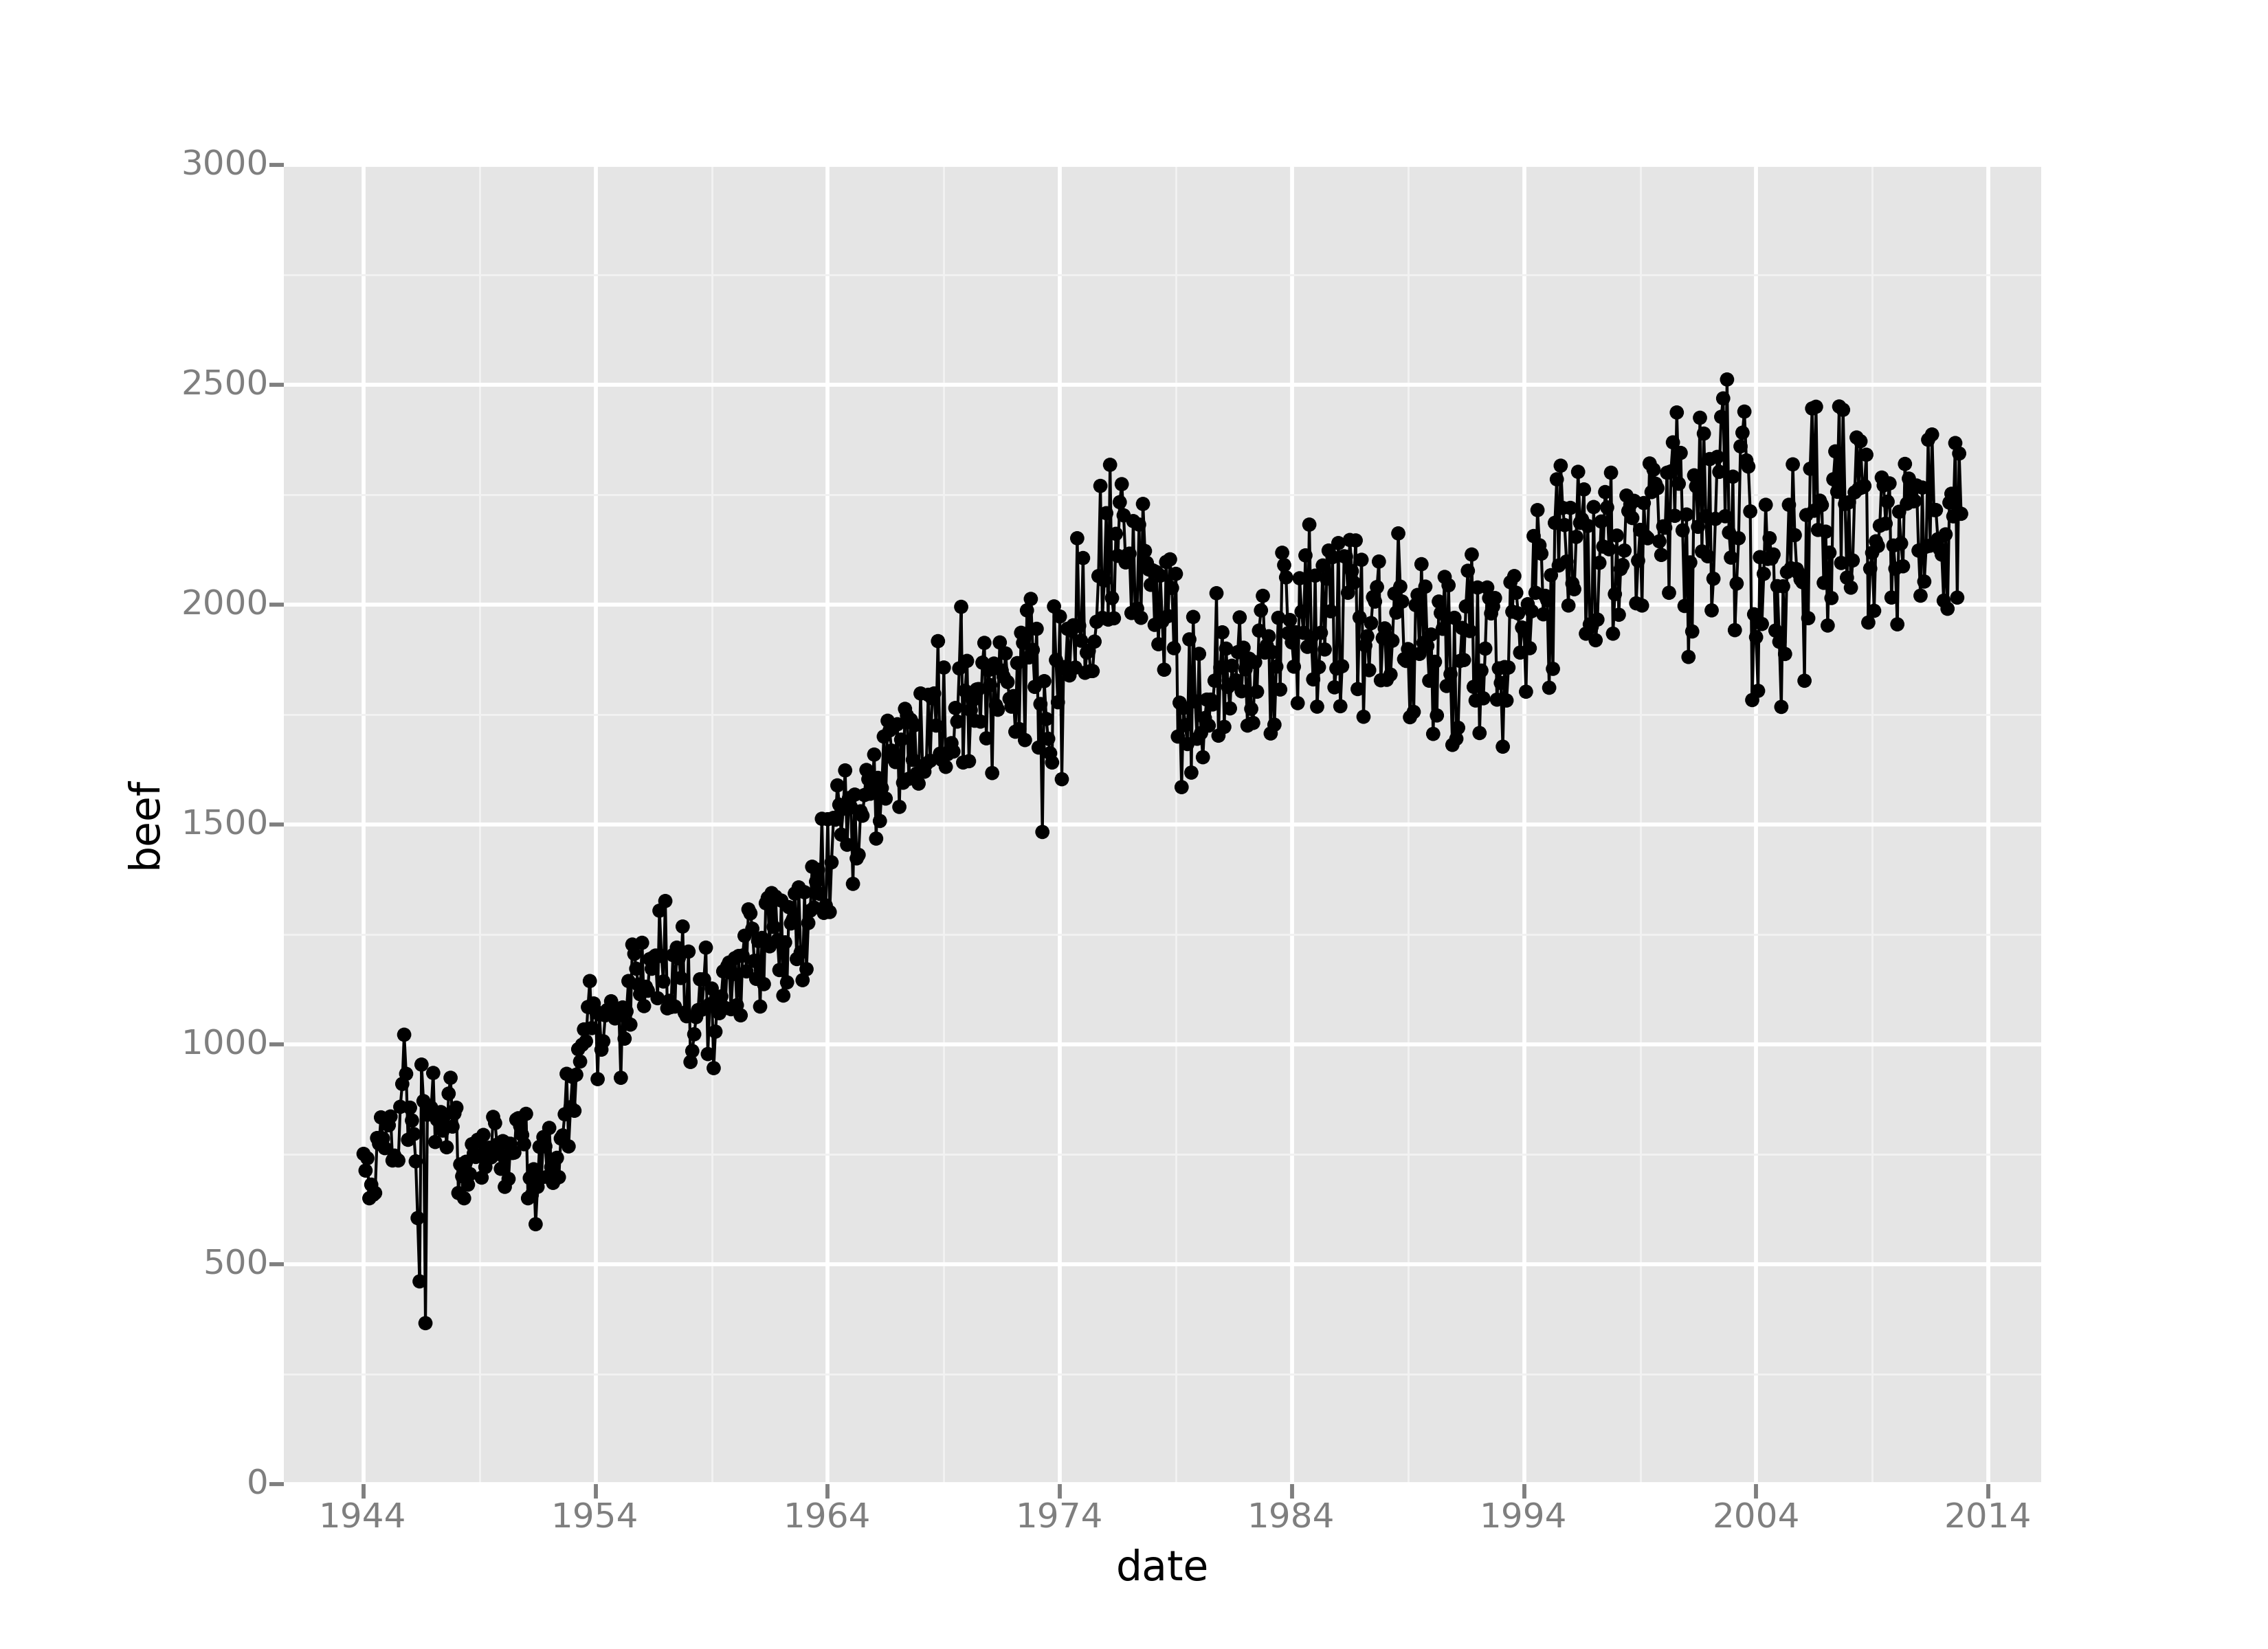
\includegraphics[width=0.7\linewidth]{Layers3}
	\end{figure}
	
\end{frame}

%================================================================================== %
\begin{frame}[fragile]
%	\frametitle{ ggplot - Layers}
\textbf{	Add a trendline.}
	\begin{framed}
		\begin{verbatim}
		p + geom_point() + geom_line() +
		stat_smooth(color="blue")
		\end{verbatim}
	\end{framed}
	\begin{figure}
		\centering
		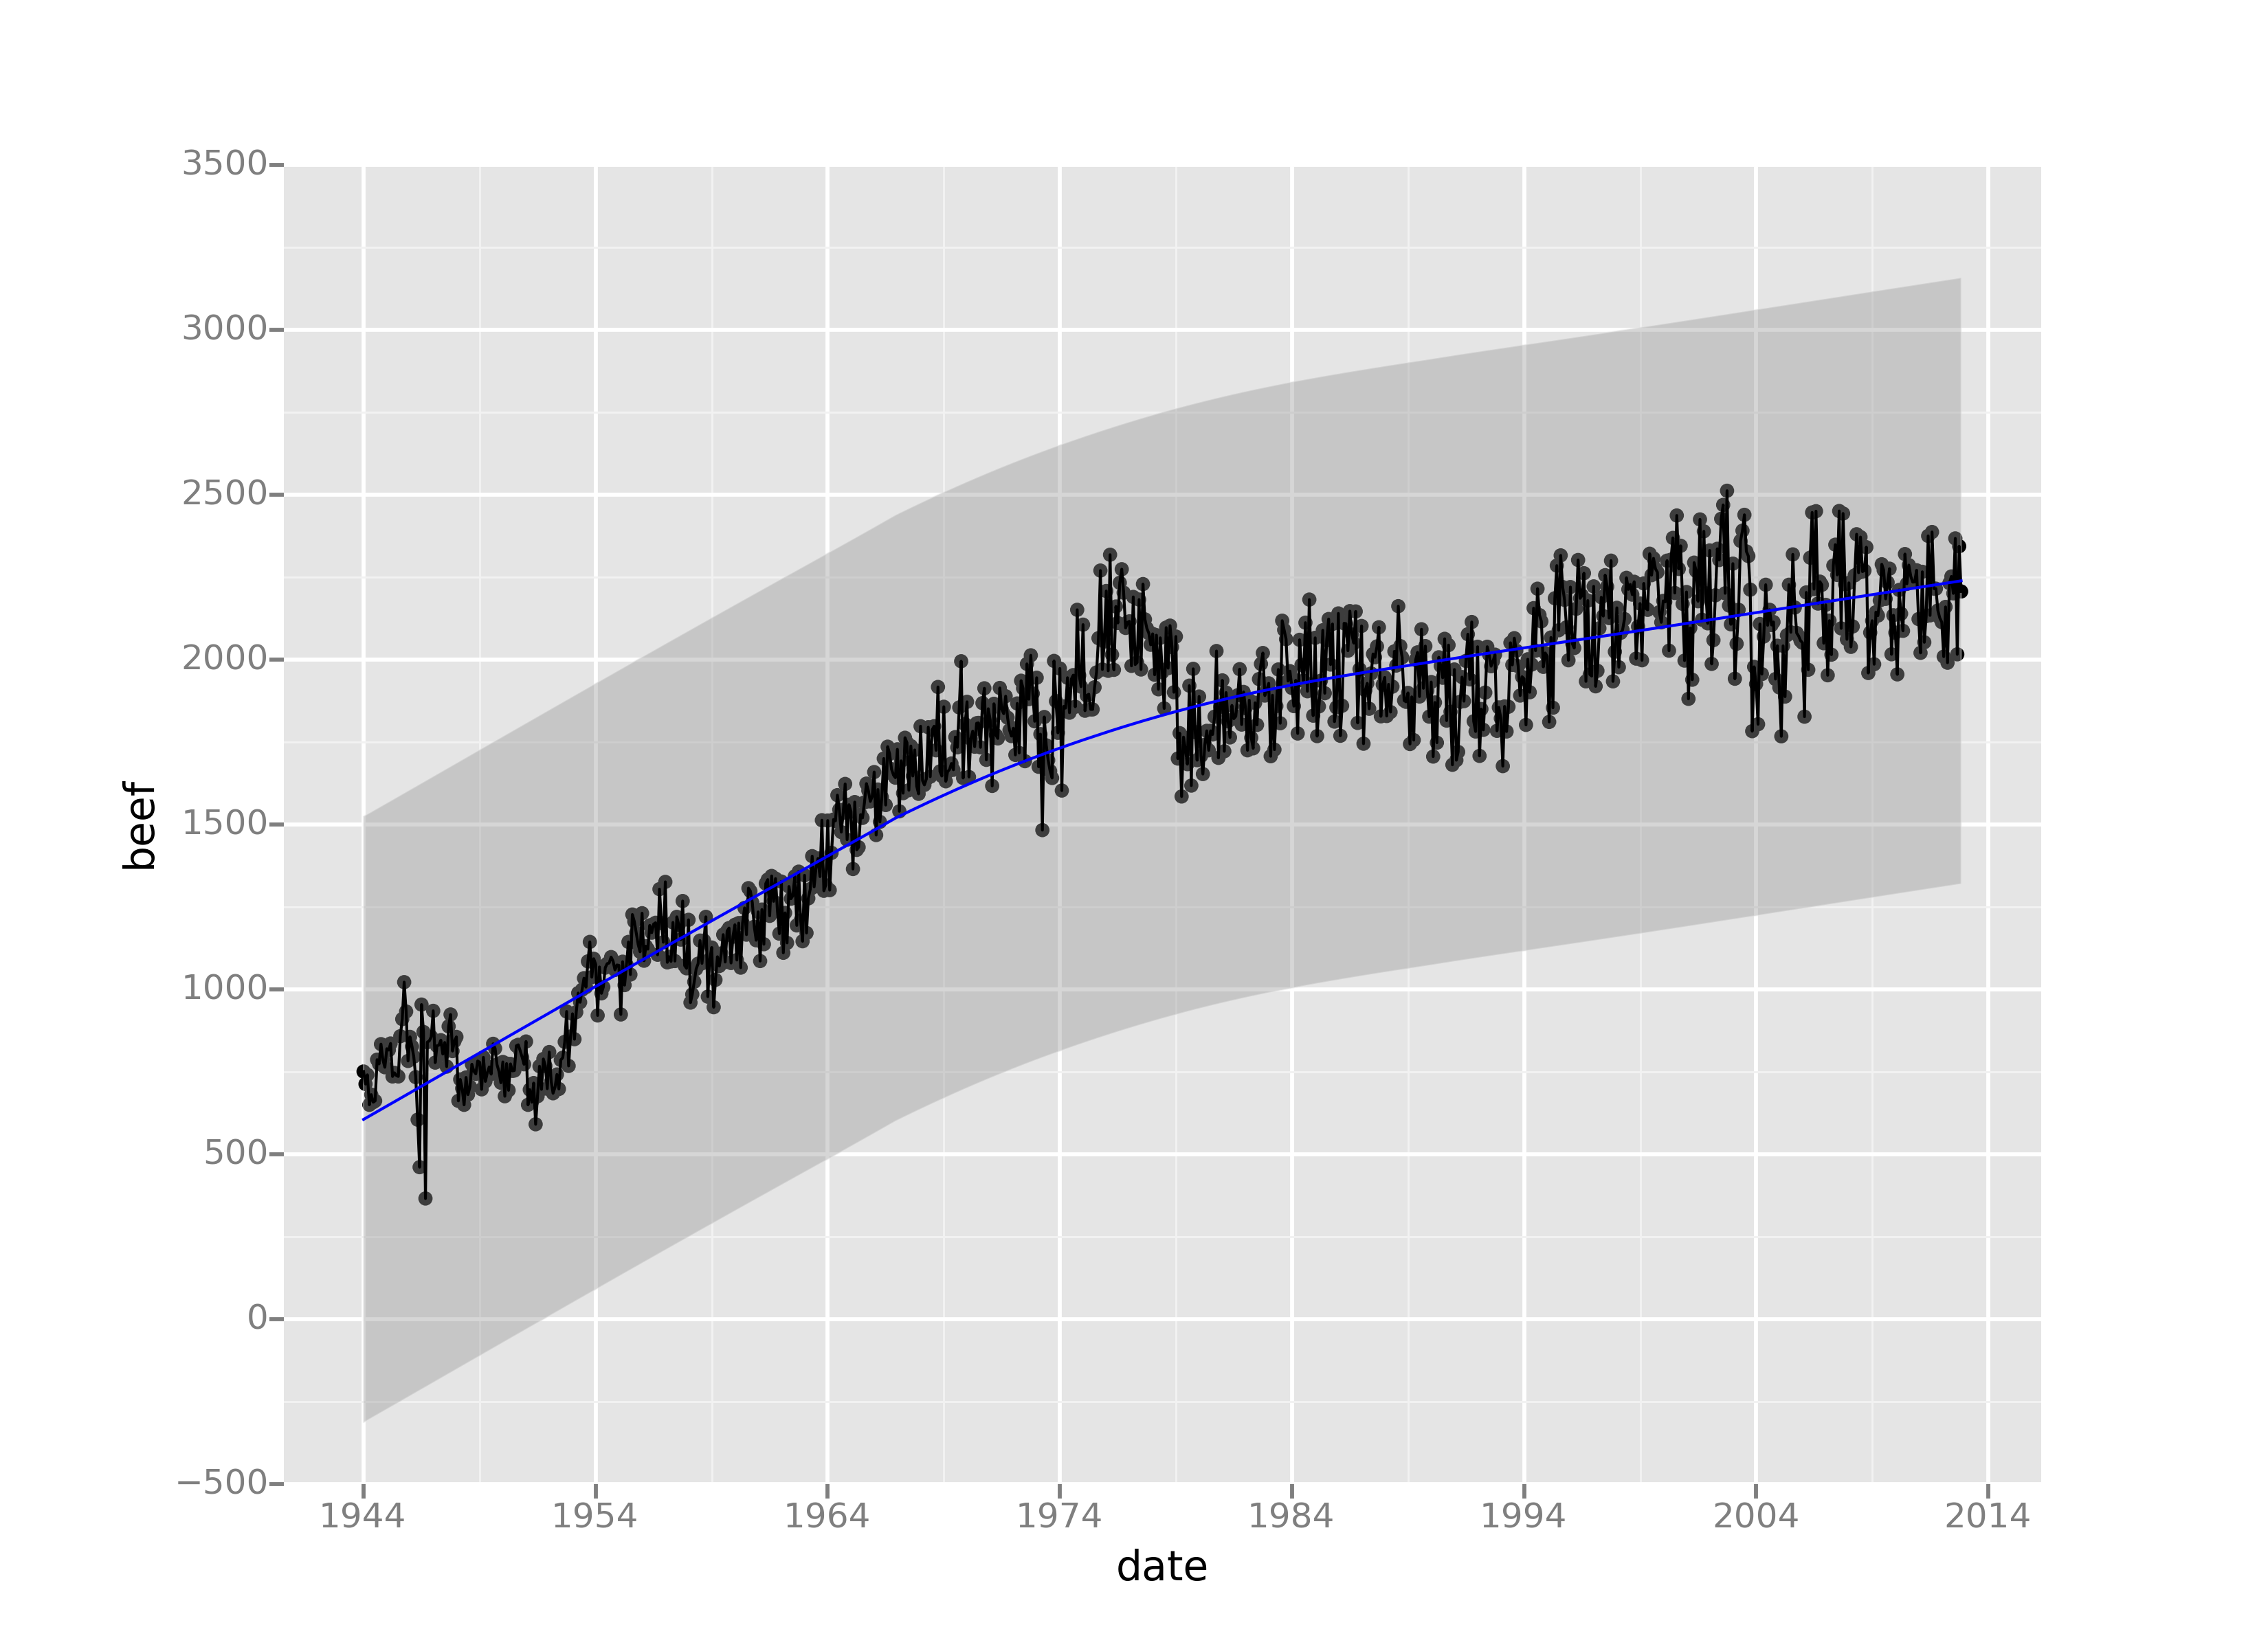
\includegraphics[width=0.7\linewidth]{layers4}
	\end{figure}
\end{frame}

\begin{frame}
\frametitle{qplot}
\Large
\begin{framed}
\begin{verbatim}
p+ ggtitle("Plot Title") + xlab(" X Axis Label") + ylab(" Y Axis Label")

\end{verbatim}
\end{framed}
\end{frame}
%================================================================================== %
\section{qplot}

\begin{frame}
\frametitle{qplot}
	\Large
\begin{itemize}
\item \texttt{qplot} is the basic plotting function in the ggplot package, designed for quick inspections of the data.
\item The functionality is not as expansive as with using ``ggplot".
\end{itemize}

\end{frame}
%=========================== %
\section{Geoms}
\begin{frame}
	\frametitle{geoms}
	\Large
	Geometric objects (geoms) are the visual representations of (subsets of) observations.
	\begin{itemize}
		\item \textbf{Univariate} - single numeric variable
		\item \textbf{Bivariate} - two numeric variable
		\item \textbf{Multivariate} - Multiple variables
	\end{itemize}
\end{frame}
%================================ %
\begin{frame}
\frametitle{geoms for ggplot}
	\Large
These are the geoms currently available for ggplot in python. \\

\bigskip
	\begin{tabular}{|l|l|l	|}
		\hline
geom\_abline	&	geom\_histogram	&	geom\_pointrange	\\ \hline
geom\_area	&	geom\_hline	&	geom\_rect	\\ \hline
geom\_bar	&	geom\_jitter	&	geom\_smooth	\\ \hline
geom\_blank	&	geom\_line	&	geom\_step	\\ \hline
geom\_boxplot	&	geom\_linerange	&	geom\_text	\\ \hline
geom\_density	&	geom\_path	&	geom\_tile	\\ \hline
geom\_dotplot	&	geom\_point	&	geom\_vline	\\ \hline


	\end{tabular} 
\end{frame}
\section{Stats}
%============================= %
\begin{frame}
\frametitle{stats}
\Large
\begin{itemize}
\item \textit{Stats} apply statistical transformations that are used to summarise the data, and allows a huge range of possibilities. \item \texttt{Stat\_smooth} is a nice stat to illustrate the principles, which fits a line and a shaded band to indicate some specified level of uncertainty, as shown in the following example which fits a linear regression line.
\end{itemize}
\end{frame}
%=============================== %
\begin{frame}[fragile]
\frametitle{stats}
\Large
\begin{framed}
\begin{verbatim}
ggplot(aes(x='date', y='beef'), data=meat) +\
geom_line() +\
stat_smooth(colour='blue', span=0.2)
\end{verbatim}
\end{framed}
\end{frame}
%================================ %
\begin{frame}
\begin{figure}
\centering
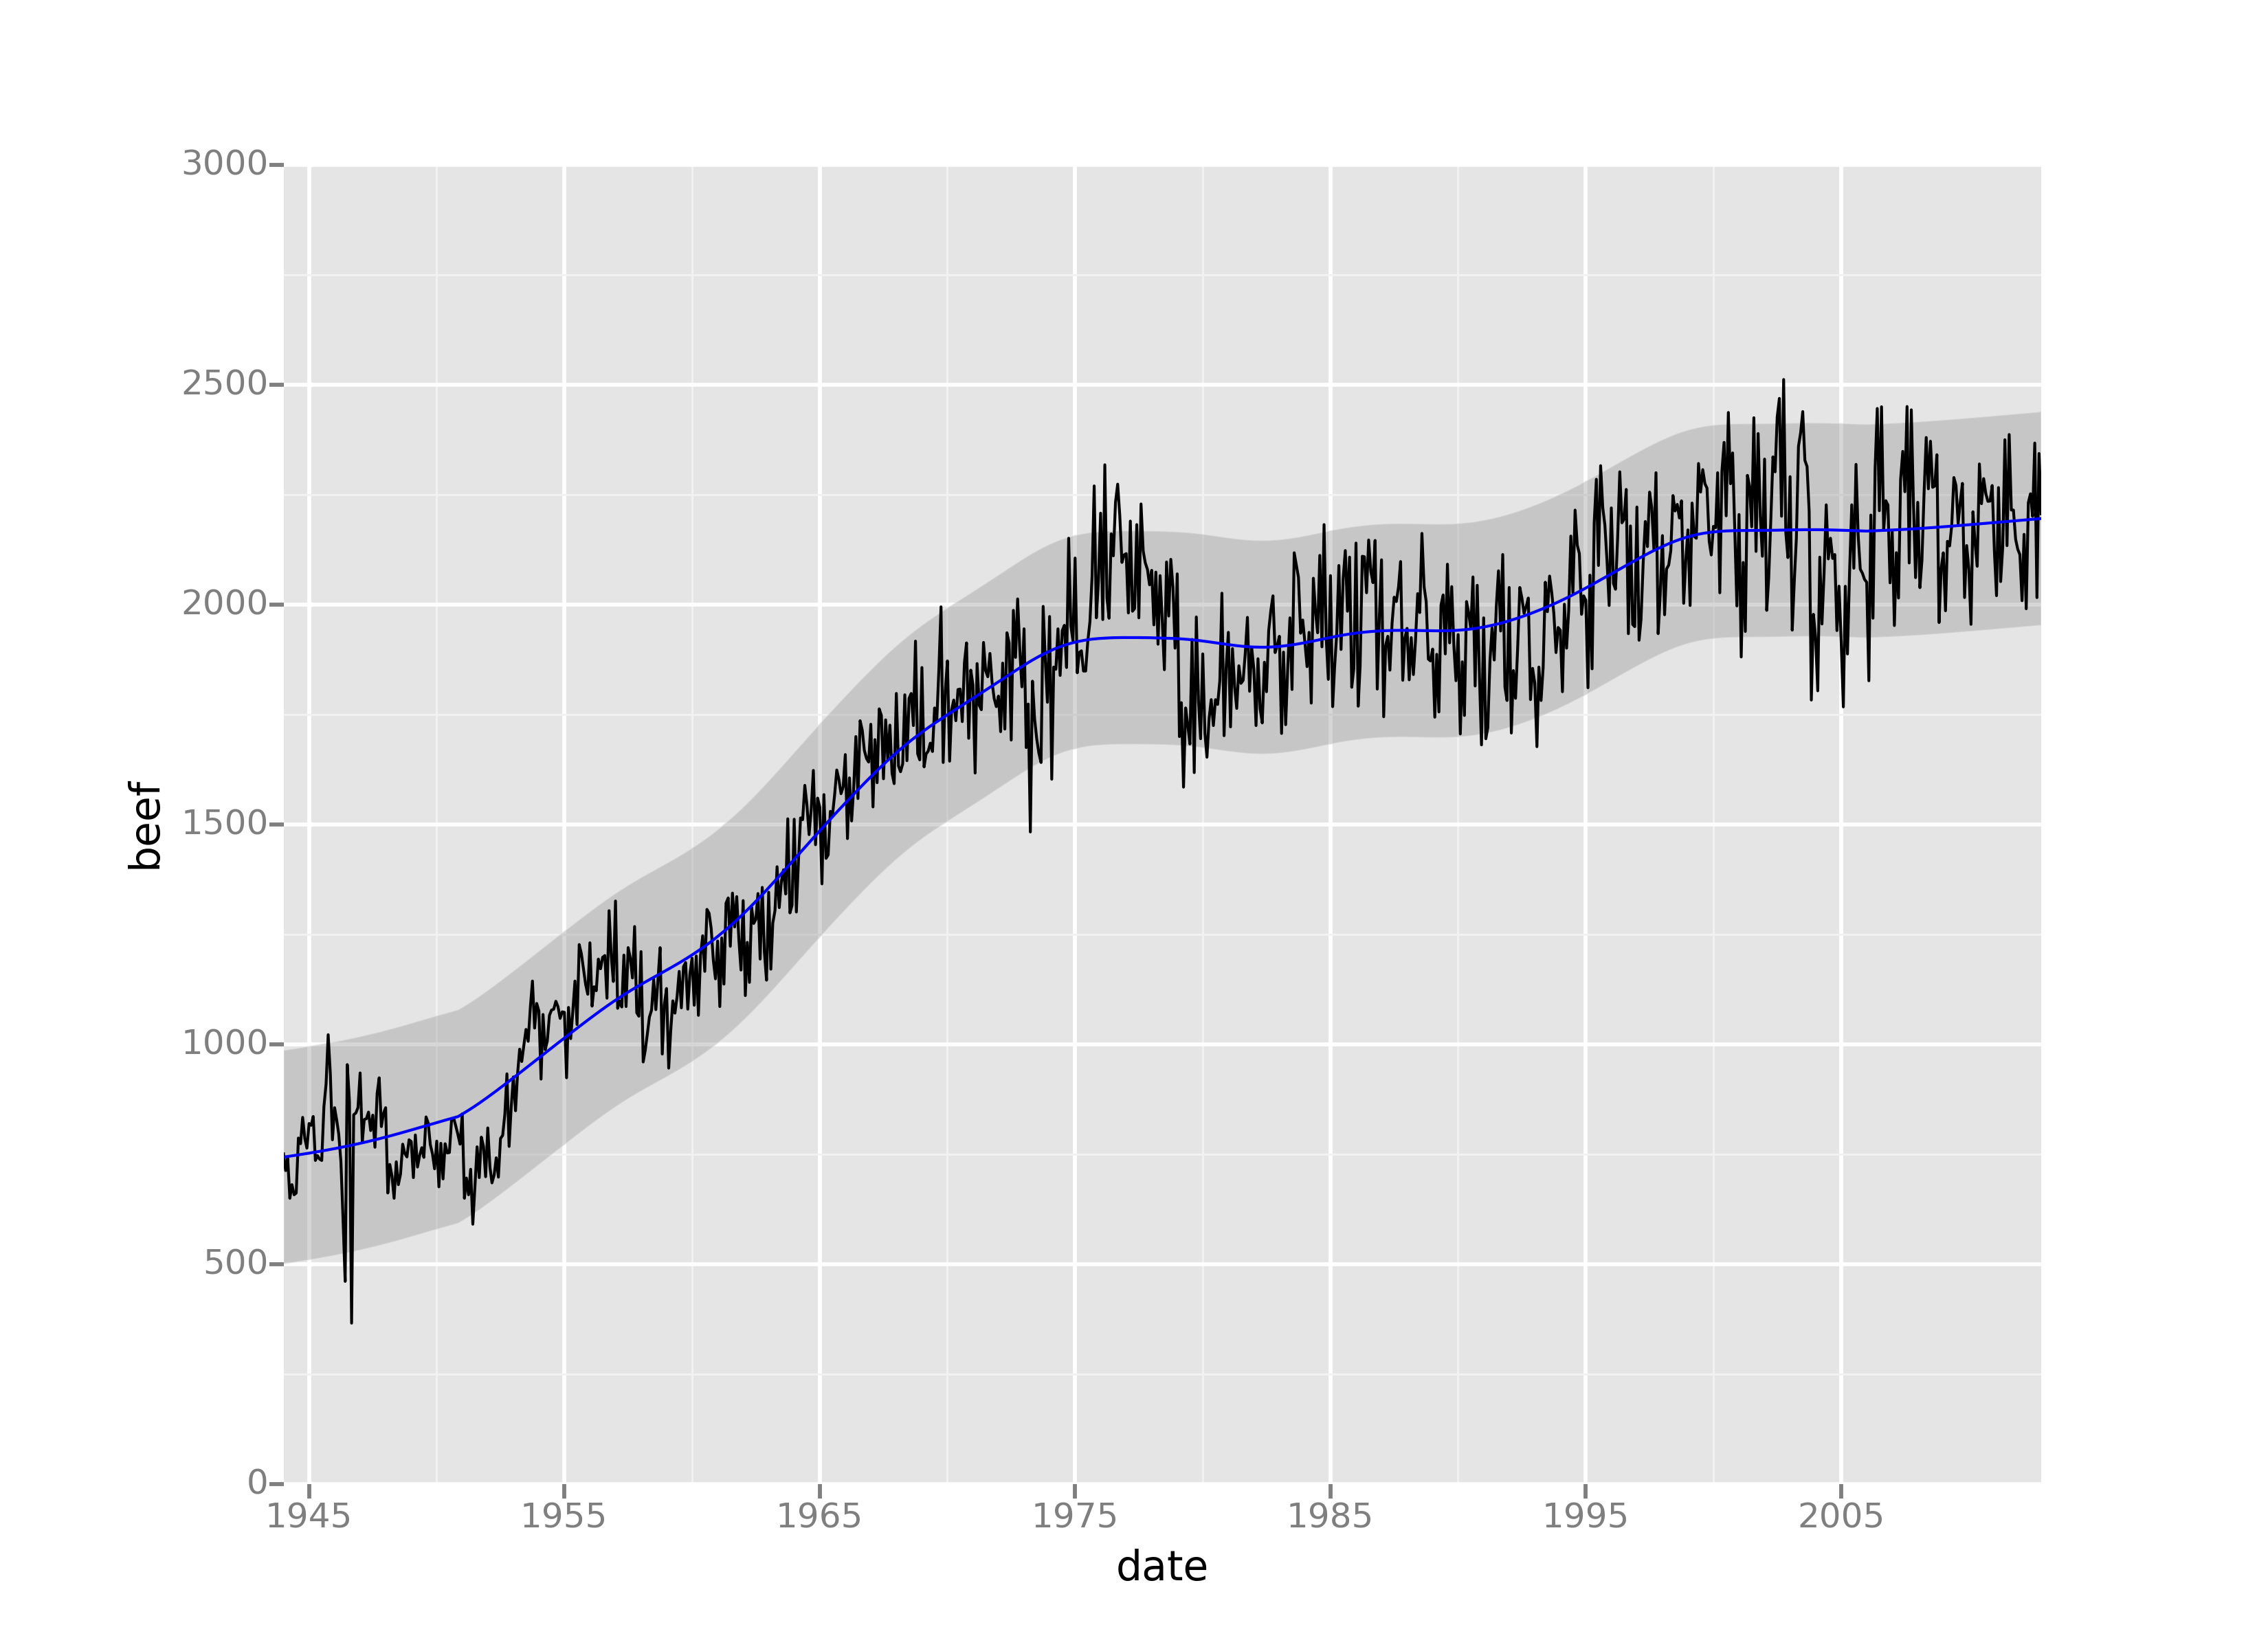
\includegraphics[width=0.7\linewidth]{stats1}
\end{figure}
\end{frame}
%==================================== %
\begin{frame}
	\frametitle{stats for ggplot}
	\Large
	These are the stats currently available for ggplot in python.\\
	\bigskip
	\begin{center}
	\begin{tabular}{|c|c|}\hline
	stat\_abline	&	stat\_hline	\\ \hline
	stat\_bar	&	stat\_identity	\\ \hline
	stat\_bin	&	stat\_smooth	\\ \hline
	stat\_bin2d	&	stat\_summary	\\ \hline
	stat\_density	&	stat\_vline	\\ \hline
	stat\_function	&		\\ \hline
	\end{tabular} 
	\end{center}
\end{frame}
%================================================ %
\begin{frame}[fragile]
	\frametitle{Aesthetics}
	\Large
	\noindent \textbf{Aesthetics}
	\begin{itemize}
		\item Aesthetics describe how your data will relate to your plots.
		\item Some common aesthetics are: \textbf{x}, \textbf{y}, and \textbf{color}. \item Aesthetics are specific to the type of plot (or layer) you're adding to your visual. 
		\item For example, a scatterplot (\texttt{geom\_point}) and a line (\texttt{geom\_line}) will share x and y, but only a line chart has a linetype aesthetic.
	\end{itemize}
	
	
	%For more information about which geoms have which aesthetics, see the DOCS SECTION.
\end{frame}
%================================================================================== %
\begin{frame}[fragile]
	\frametitle{Aesthetics}
	\Large
Aesthetics correspond with the ``X" and ``Y" variables. The first line of the code below indicates which variable is which.
\begin{framed}
\begin{verbatim}
ggplot(aes(x="date",y="beef"), meat) +\
geom_line() +\
stat_smooth(colour="blue", span=0.2)
\end{verbatim}
\end{framed}

\end{frame}
%================================================================================== %
\begin{frame}[fragile]
	\frametitle{Aesthetics}
	\Large
The first aesthetic variable is for \texttt{color}. This can be used to depict subcategories in the data.
	\begin{framed}
		\begin{verbatim}
ggplot(diamonds, aes(x="carat", 
  y="price", color="cut")) +\
  geom_point() +\ ....
	\end{verbatim}
\end{framed}

\end{frame}
%================================================================================== %
\begin{frame}
	
	\begin{figure}
\centering
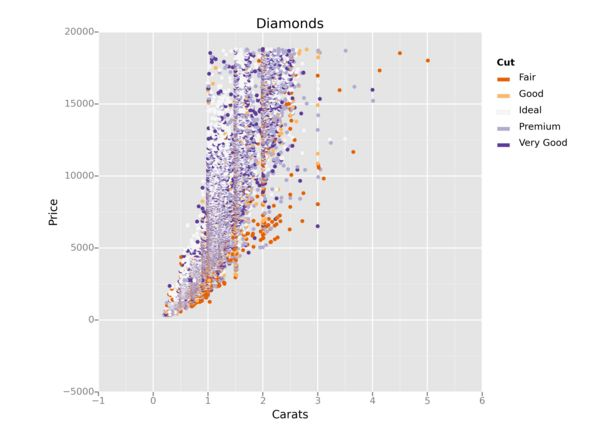
\includegraphics[width=1.1\linewidth]{aesthetic2}
\end{figure}

\end{frame}
%================================================================================== %
\section{Faceting}






\begin{frame}
	\Large
	\noindent \textbf{Faceting}\\
	The faceting approach supported by ggplot partitions a plot into a matrix of panels. Each panel shows a different subset of the data.
	There are two faceting approaches:
	
	\begin{itemize}
		\item \texttt{facet\_wrap("cell")} - univariate: create a 1-d strip of panels, based on one factor, and wrap the strip into a 2-d matrix
		\item \texttt{facet\_grid("row","col")} - (usually) bivariate: create a 2-d matrix of panels, based on two factors
	\end{itemize}
\end{frame}
%================================ %
\begin{frame}[fragile]
	\frametitle{Faceting}
\Large
Suppose \texttt{cyl} and \texttt{drv} are two categorical variables in a data frame
\begin{framed}
\begin{verbatim}
qplot(.....) + facet_grid("cyl","drv")
\end{verbatim}
\end{framed}

\end{frame}
%================================ %
\begin{frame}
	\frametitle{Faceting}
	\begin{figure}
\centering
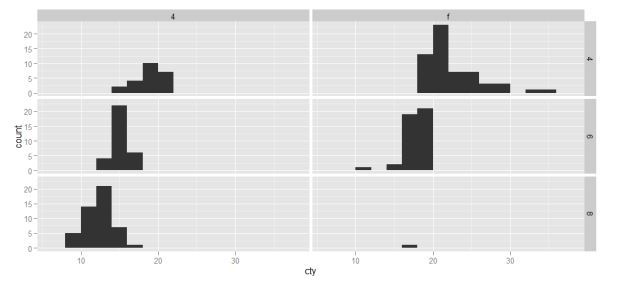
\includegraphics[width=1.1\linewidth]{gridfacetting}
\caption{Grid Faceting}
\label{fig:gridfacetting}
\end{figure}

\end{frame}



%================================ %
\begin{frame}
	\frametitle{Faceting}
\Large
\vspace{-1cm}
\noindent \textbf{Facet Wrap}
\begin{itemize}
\item An alternative to grid facetting is a wrapped ribbon of plots
\item \texttt{facet\_wrap} generates a long ribbon of plots, and wraps it into 2d.
\end{itemize}

\end{frame}
%
%\begin{frame}
%	\begin{figure}
%\centering
%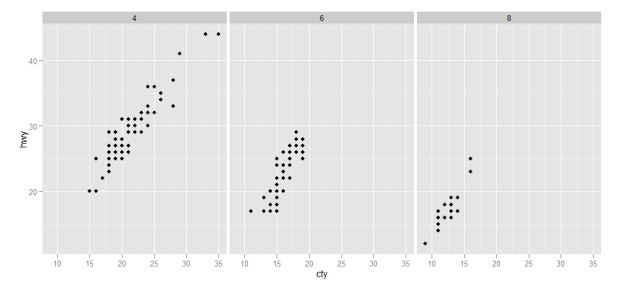
\includegraphics[width=1.1\linewidth]{FacetWrap}
%\caption{Facet Wrap}
%\label{fig:FacetWrap}
%\end{figure}
%
%\end{frame}



%========================== %
\begin{frame}[fragile]
	% % Faceting 1
	\frametitle{Faceting}
	\Large 
	\noindent \textbf{Facetting - Examples}
{
	\large
	\begin{framed}
		\begin{verbatim}
p = ggplot(aes(x="date", y="value"), data=meat2)

# Scatterplot with Smoother
p + geom_point() + \
stat_smooth(colour="red") + \
facet_wrap("variable")
		\end{verbatim}
		
	\end{framed}
}
\end{frame}
%================================== %\
\begin{frame}
\frametitle{Faceting}
	
	\begin{figure}
		\centering
		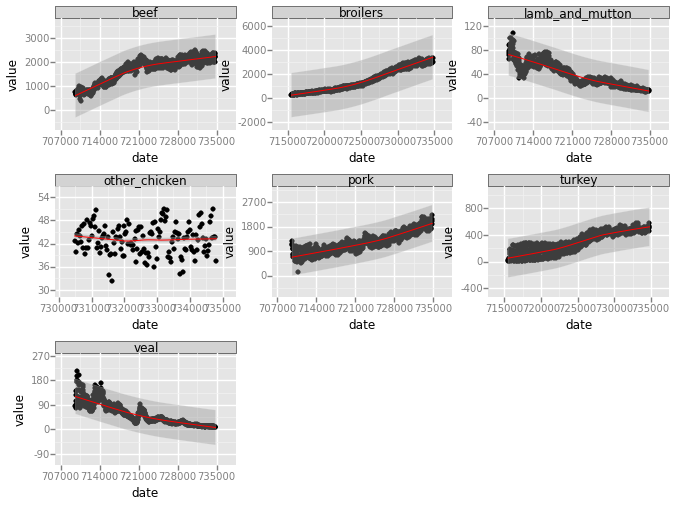
\includegraphics[width=1.0\linewidth]{Facet1}
		\caption{}
		\label{fig:Facet1}
	\end{figure}
	
\end{frame}
%========================== %
\begin{frame}[fragile]
	% % Faceting 2
	\frametitle{Faceting}
\Large
	\begin{framed}
		\begin{verbatim}
p = ggplot(aes(x="price"), data=diamonds)
p + geom_histogram() + facet_wrap("cut")
		\end{verbatim}
		
	\end{framed}
\end{frame}

%================================== %\
\begin{frame}
	\begin{figure}
		\centering
		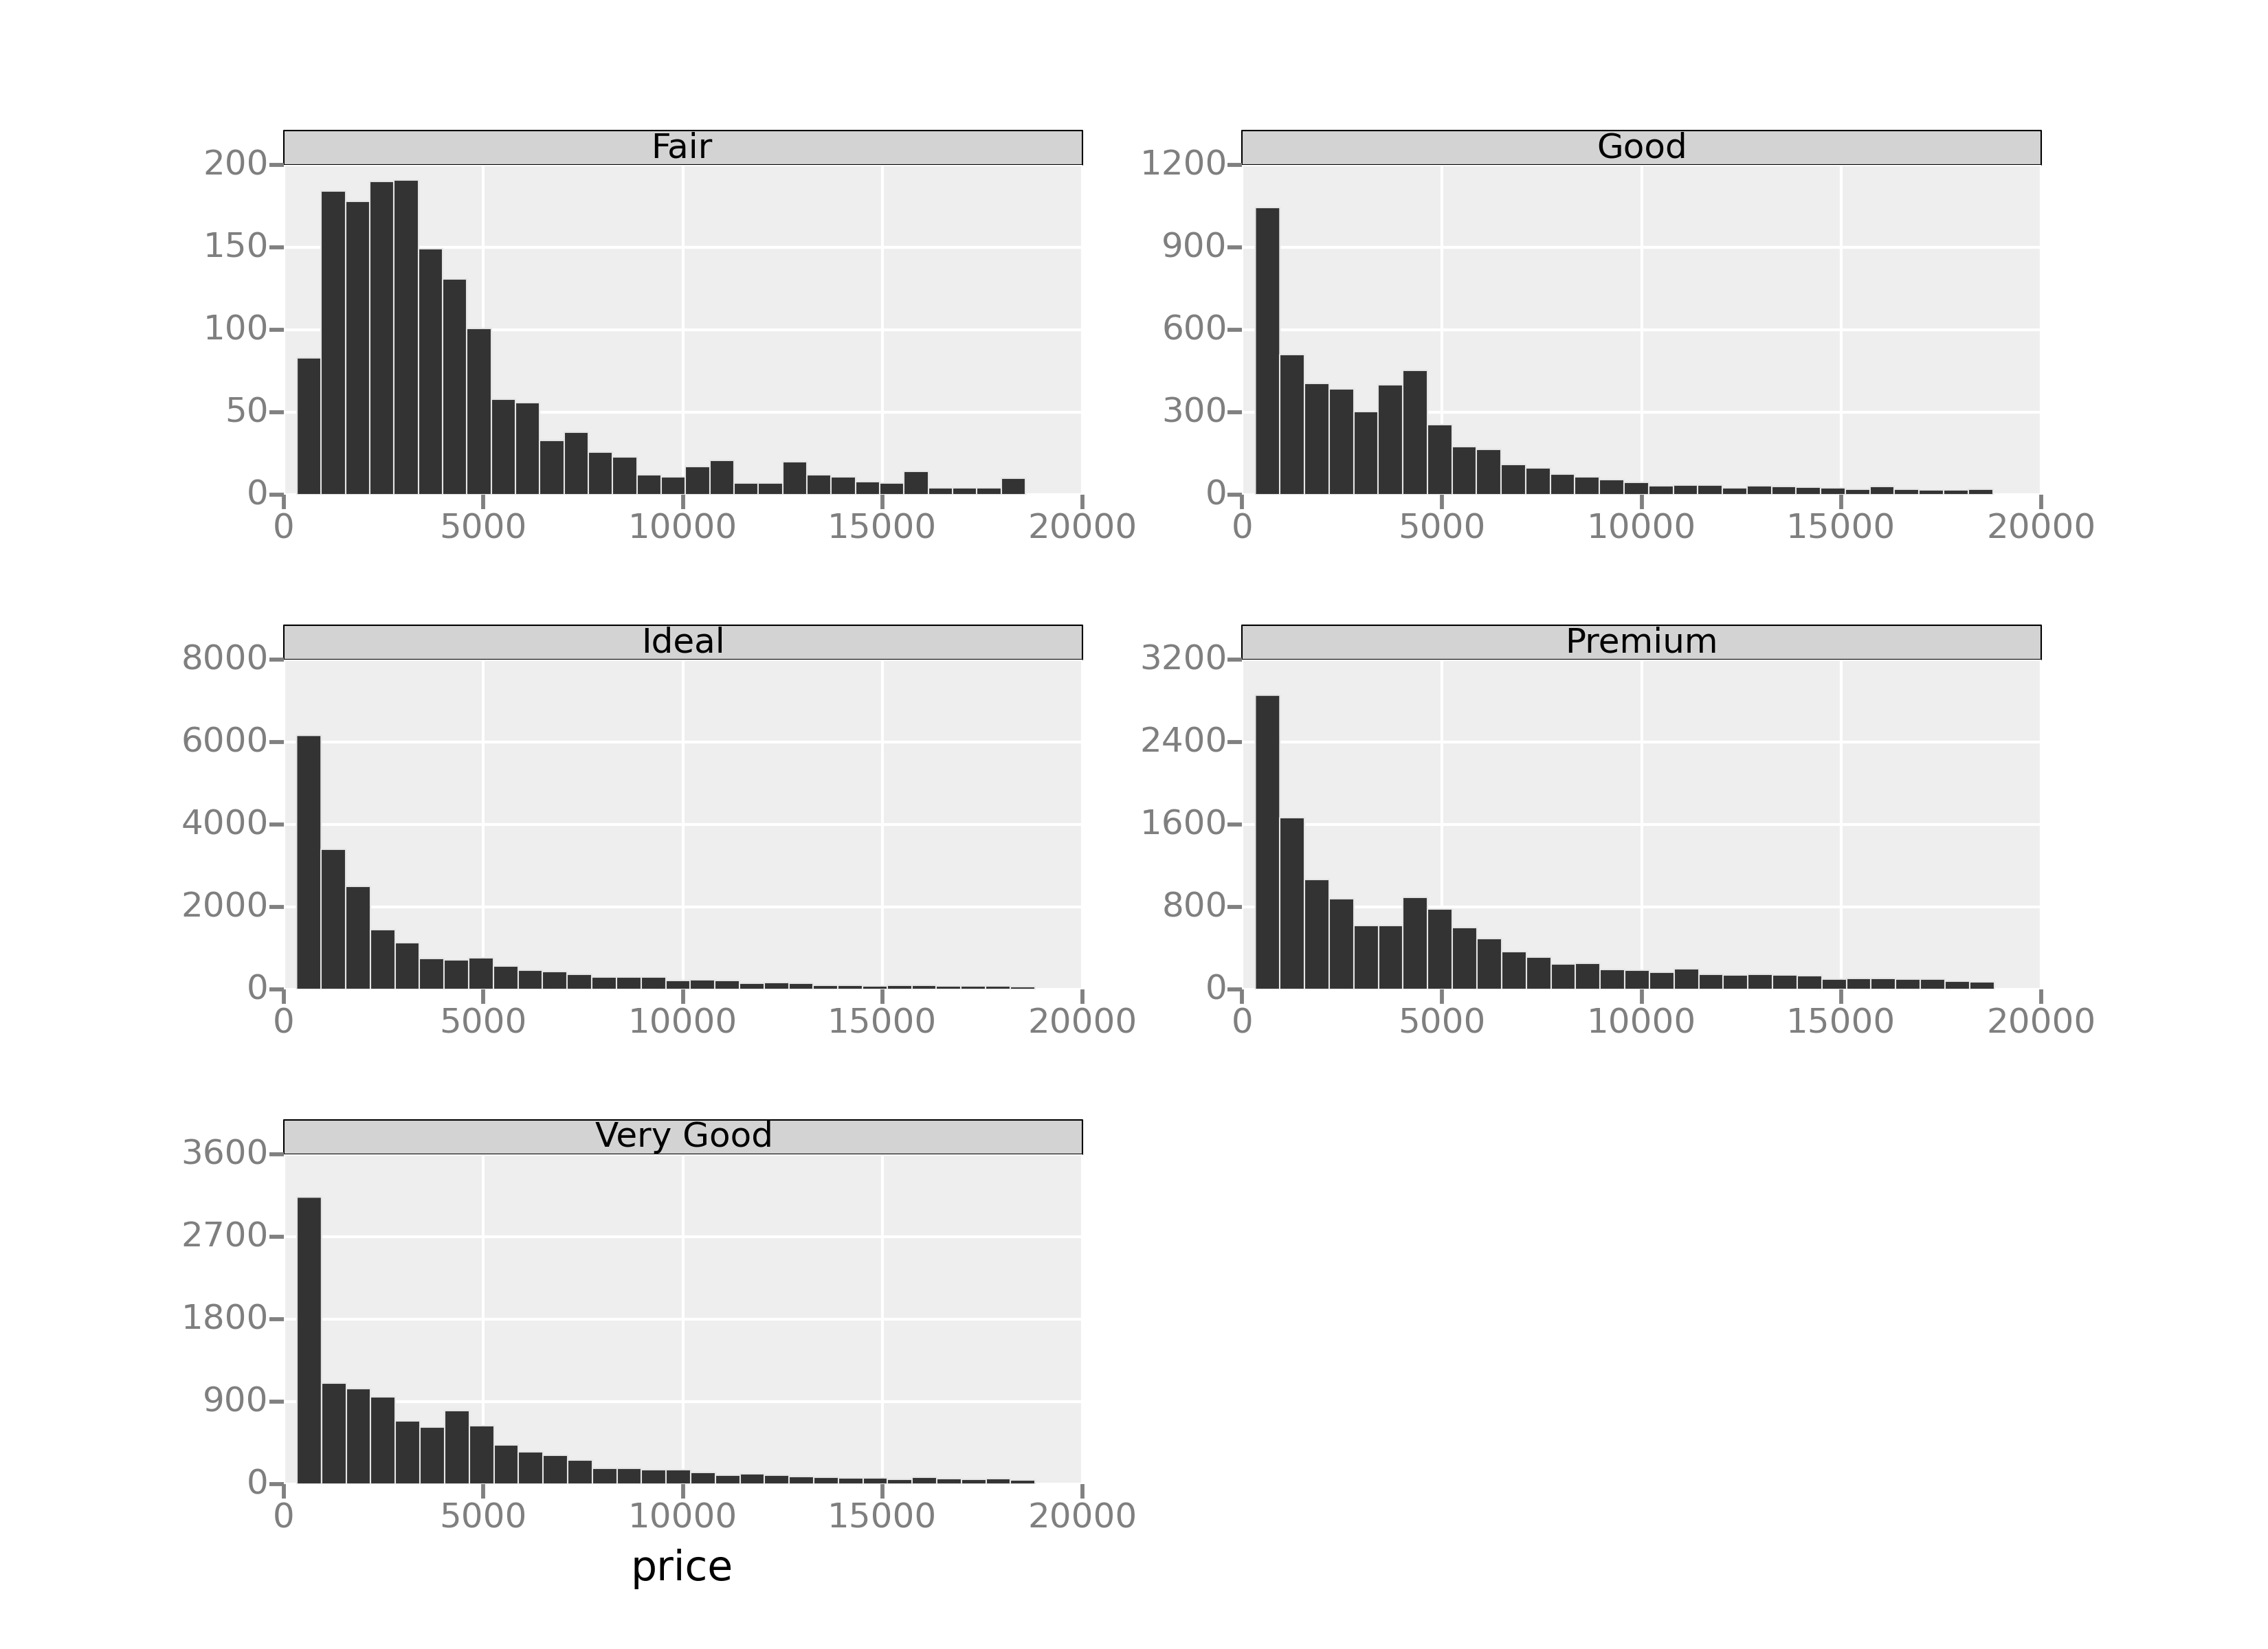
\includegraphics[width=0.7\linewidth]{FacetsB}
		\caption{}
		\label{fig:FacetsB}
	\end{figure}
	
\end{frame}

%========================== %
\begin{frame}[fragile]
	% % Faceting 3
	\frametitle{Faceting}
	\begin{framed}
		\begin{verbatim}
p = ggplot(diamonds, aes(x='price'))
p + geom_density() + \
facet_grid("cut", "clarity")
		\end{verbatim}
		
	\end{framed}
\end{frame}
%================================== %\
\begin{frame}
\frametitle{Faceting}
	\begin{figure}
		\centering
		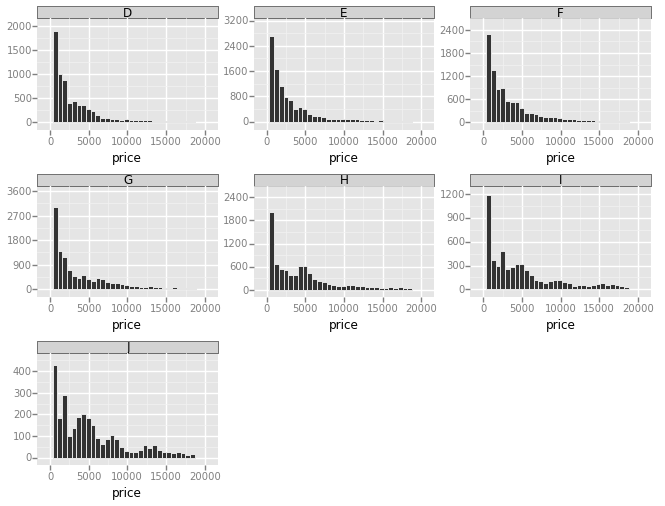
\includegraphics[width=0.7\linewidth]{Facet3}
		\caption{}
		\label{fig:Facet3}
	\end{figure}
	
\end{frame}
%========================== %
\begin{frame}[fragile]
\frametitle{Faceting}
	\begin{framed}
		\begin{verbatim}
p = ggplot(diamonds, aes(x='carat', y='price'))
p + geom_point(alpha=0.25) + \
facet_grid("cut", "clarity")
	\end{verbatim}
	
\end{framed}
\end{frame}
%========================== %
\begin{frame}
\frametitle{Faceting}
	\begin{figure}
\centering
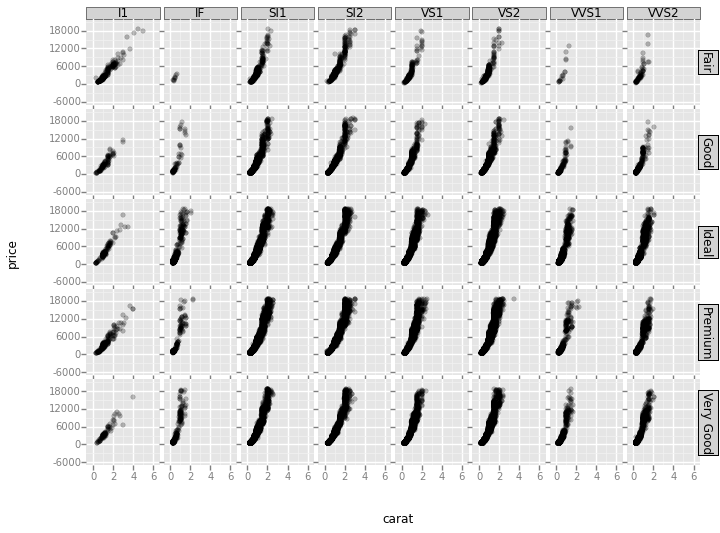
\includegraphics[width=0.99\linewidth]{Facet4}
\end{figure}

\end{frame}
%========================== %
\begin{frame}[fragile]
	\begin{framed}
	\begin{verbatim}
p  = ggplot(iris, aes("Sepal.Length", "Sepal.Width"))
p + geom_boxplot(fill = c("lightblue")) + facet_wrap("Species")

	\end{verbatim}
		
	\end{framed}
\end{frame}



\begin{frame}
	\begin{figure}
		\centering
		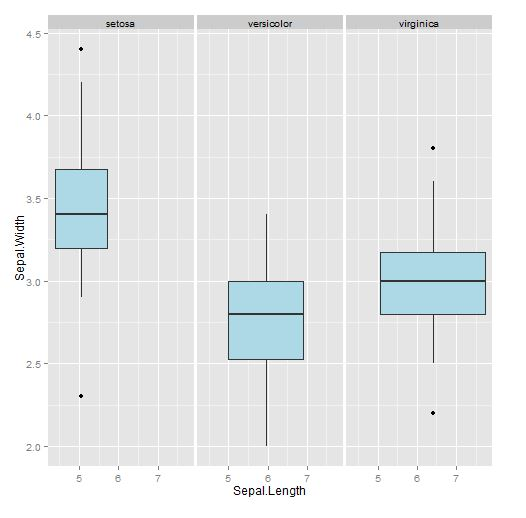
\includegraphics[width=0.7\linewidth]{iris-boxplot}
		\caption{}
		\label{fig:iris-boxplot}
	\end{figure}
	
\end{frame}

%================================= %
\section*{Scales}
% http://sape.inf.usi.ch/quick-reference/ggplot2/scale
\begin{frame}
\noindent \textbf{Scales and Themes}
	\begin{itemize}
	\item ggplot2 provides a large number of scale functions
	to control aspects of a graphic including axes and
	legends
	\item theme functions allow us to control the overall style
	of the graphic
	\end{itemize}

\end{frame}

\begin{frame}
	\Large
	\noindent \textbf{Scales}
	\begin{itemize}
		\item A scale determines how an attribute of the data is mapped into an aesthetic property of a \texttt{geom} (e.g., the geom's position along the x axis, or a geom's fill color in a color space).
		\item The colours and shapes used in the chart can be manually adjusted if you don’t like the defaults.
	\end{itemize}
	
\end{frame}
%================================== %
\section{Themes}
\begin{frame}[fragile]
\frametitle{Themes}
\Large
	\begin{framed}
	\begin{verbatim}
	ggplot(aes(x="date", y="beef"),meat) +\
	geom_line() +\
	theme_bw()
	\end{verbatim}
	\end{framed}
\end{frame}
%============================ %
\begin{frame}
\frametitle{Themes}
\Large
\begin{figure}
\centering
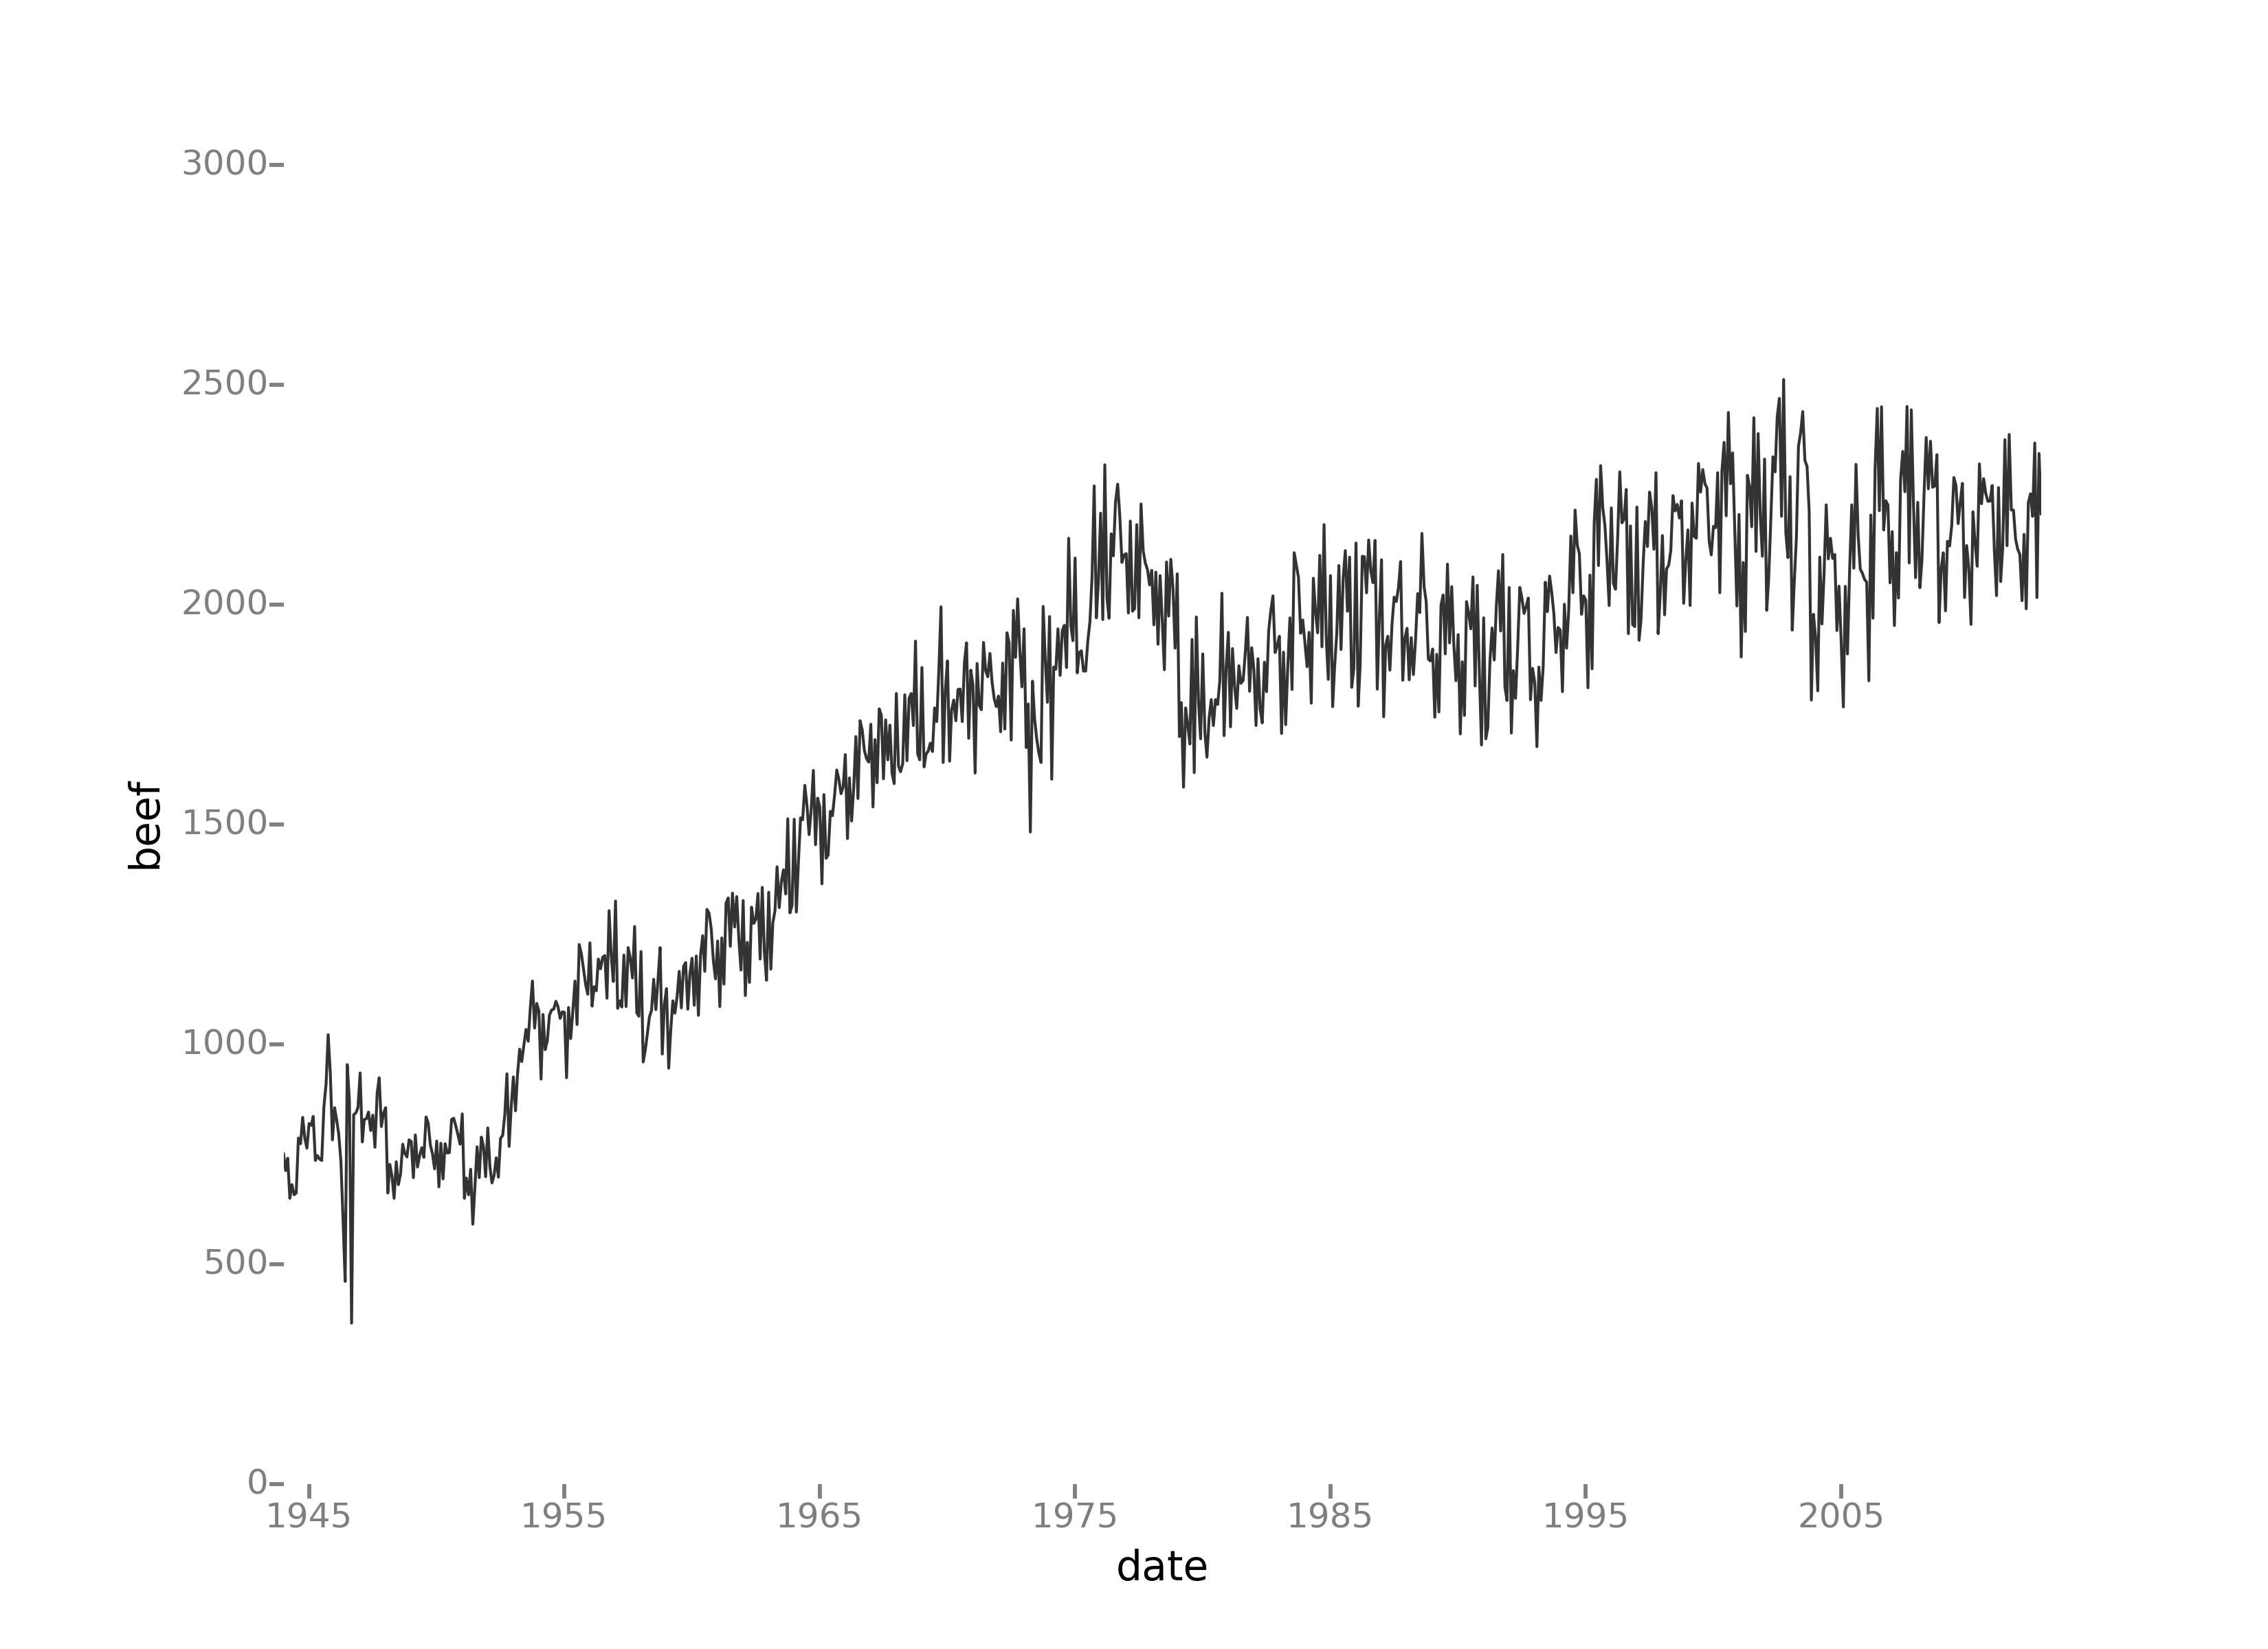
\includegraphics[width=1.0\linewidth]{meat_theme_bw}
\end{figure}

\end{frame}
\begin{frame}
\frametitle{Themes}
\Large
Try out the following themes
	\begin{itemize}
		\item	\texttt{theme\_538}
		\item	\texttt{theme\_bw}
		\item	\texttt{theme\_gray}
		\item	\texttt{theme\_matplotlib}
		\item	\texttt{theme\_seaborn}
		\item	\texttt{theme\_xkcd}
	\end{itemize}
	
\end{frame}
\end{document}
